% cuRAMSES: Scalable Domain Decomposition and CUDA-enabled AMR
% for Cosmological Simulations
%
% MNRAS-style LaTeX paper
%
\documentclass[fleqn,usenatbib]{mnras}

% Standard packages
\usepackage{amsmath,amssymb}
\usepackage{graphicx}
\usepackage{algorithm}
\usepackage{algorithmic}
\usepackage{booktabs}
\usepackage{multirow}
\usepackage{xcolor}
\usepackage{hyperref}
\usepackage{lineno}

% Algorithm formatting
\renewcommand{\algorithmicrequire}{\textbf{Input:}}
\renewcommand{\algorithmicensure}{\textbf{Output:}}

% Shorthand macros
\newcommand{\ramses}{\textsc{ramses}}
\newcommand{\curamses}{\textsc{cuRAMSES}}
\newcommand{\ncpu}{N_{\rm cpu}}
\newcommand{\ngridmax}{N_{\rm gridmax}}
\newcommand{\nlevelmax}{N_{\rm levelmax}}
\newcommand{\twotondim}{2^{N_{\rm dim}}}
\newcommand{\ksec}{\ensuremath{k}\text{-section}}
\newcommand{\Olog}[1]{\mathcal{O}(#1)}
\newcommand{\code}[1]{\texttt{#1}}

\title[cuRAMSES: Scalable CUDA-enabled AMR for Cosmological Simulations]
{cuRAMSES: Scalable Domain Decomposition and CUDA-enabled AMR
for Cosmological Simulations}

\author[J.~Kim]{
Juhan Kim$^{1}$\thanks{E-mail: kjhan@kias.re.kr}
\\
$^{1}$Center for Advanced Computation, Korea Institute for Advanced Study,
85 Hoegiro, Dongdaemun-gu, Seoul 02455, Republic of Korea
}

\date{Accepted XXX. Received YYY; in original form ZZZ}

\pubyear{2026}

\begin{document}
\linenumbers

\label{firstpage}
\pagerange{\pageref{firstpage}--\pageref{lastpage}}

\maketitle

% ===================================================================
% ABSTRACT
% ===================================================================
\begin{abstract}
We present \curamses, a suite of algorithmic and implementation
improvements to the \ramses\ adaptive mesh refinement (AMR)
cosmological simulation code that address the principal bottlenecks
encountered in large-scale simulations: communication overhead, memory
consumption, and solver efficiency. The central innovation is a
recursive \ksec\ domain decomposition that replaces the traditional
Hilbert curve ordering with a hierarchical spatial partitioning,
dramatically reducing the number of MPI messages per ghost-zone
exchange and eliminating all \code{MPI\_ALLTOALL} calls. A Morton key
hash table for octree neighbour lookup removes one of the largest
per-rank arrays in the original code, while on-demand allocation
strategies for auxiliary arrays further reduce the memory footprint.
A hybrid CPU/GPU dispatch model offloads the Godunov solver and
multigrid Poisson solver to CUDA streams at runtime, using
GPU-resident mesh data and halo-only PCIe transfers to minimise
host--device overhead; automatic fallback to CPU execution is provided
when GPU memory is insufficient. We also implement variable-$\ncpu$ restart for both HDF5 and
native binary output formats, removing the constraint that
output files must be read with the same number of MPI ranks as
were used to write them. All modifications preserve
physical consistency, as verified by conservation-law diagnostics
across extensive test suites.
\end{abstract}

\begin{keywords}
methods: numerical -- cosmology: simulations -- hydrodynamics --
software: development
\end{keywords}

% ===================================================================
% 1. INTRODUCTION
% ===================================================================
\section{INTRODUCTION}
\label{sec:intro}

Cosmological hydrodynamic simulations play a central role in modern
astrophysics, connecting the predictions of the $\Lambda$CDM paradigm
to the observable properties of galaxies, the intergalactic medium,
and the large-scale structure of the Universe. Over the past decade,
a series of landmark galaxy formation simulations have advanced our
understanding of cosmic structure: the Illustris and IllustrisTNG
projects \citep{Vogelsberger2014,Pillepich2018,Nelson2019} using the
moving-mesh code \textsc{arepo} \citep{Springel2010}, the EAGLE
simulation \citep{Schaye2015} with the smoothed-particle hydrodynamics
code \textsc{gadget} \citep{Springel2005}, the Horizon-AGN simulation
\citep{Dubois2014} and its high-resolution successor NewHorizon
\citep{Dubois2021} using the adaptive mesh refinement (AMR) code
\ramses\ \citep{Teyssier2002}, and the FIRE project
\citep{Hopkins2018} with the meshless finite-mass code \textsc{gizmo}
\citep{Hopkins2015}.

Among the numerical approaches employed by these simulations, AMR
codes such as \ramses\ and Enzo \citep{Bryan2014} provide a
particularly attractive framework: the
computational mesh is refined only where the physics demands it,
concentrating resources on collapsing haloes and star-forming regions
while keeping the cost of smooth, low-density regions manageable.

A key design choice in parallel AMR codes is the domain decomposition
strategy. Space-filling curves (SFCs), particularly the Hilbert
(Peano--Hilbert) curve, have been widely adopted for this purpose
\citep{Warren1993,Springel2005}. The Hilbert curve maps the
three-dimensional computational domain to a one-dimensional index,
preserving spatial locality so that cells close in physical space
remain close along the curve. This enables a simple and effective
partitioning: the one-dimensional index range is divided into $\ncpu$
contiguous segments, each assigned to an MPI rank. The resulting
decomposition naturally produces compact subdomains with relatively
small surface-to-volume ratios, minimising the ghost-zone boundary
between neighbouring ranks.

However, scaling this approach to the regime of $10^{10}$--$10^{11}$
particles and $10^4$--$10^5$ MPI ranks reveals fundamental
limitations. The one-dimensional nature of the SFC means that
\emph{every} rank may, in principle, border \emph{any other} rank,
forcing communication patterns that scale poorly with $\ncpu$. In the
standard \ramses\ implementation, ghost-zone exchange, grid and particle migration, and sink particle
synchronisation all rely on \code{MPI\_ALLTOALL} to communicate
counts among all ranks, leading to $\Olog{\ncpu^2}$ message
complexity and $\Olog{\ncpu}$ per-rank buffer memory --- a severe
bottleneck when $\ncpu$ exceeds ${\sim}10^3$
\citep{Teyssier2002}. Furthermore, the Hilbert ordering distributes
load based on cell count alone, which becomes increasingly inadequate
for cosmological simulations where the particle distribution is highly
clustered: a cell hosting $10^4$ particles in a dense halo is far more
expensive in memory than a void cell with zero particles, yet the
standard load balancer treats them equally
\citep{Springel2005}. The problem is particularly acute in
cosmological zoom-in simulations \citep{Dubois2021}, where the
high-resolution region occupies a small fraction of the total volume:
the Hilbert curve concentrates nearly all refinement on a few ranks
while the remaining ranks are left with low-resolution void cells,
leading to severe load imbalance that worsens with increasing zoom
factor.

Beyond the communication and load-balancing challenges, several other
bottlenecks arise. Large per-rank arrays scale linearly with
$\ngridmax$: the neighbour-pointer array \code{nbor($\ngridmax$, 6)}
alone consumes $48\,\ngridmax$ bytes \citep{Teyssier2002}, and the
Hilbert key array adds another $16\,\ngridmax$ bytes (when compiled
with \code{QUADHILBERT}), together approaching 1\,GB per rank for
production configurations with $\ngridmax \sim 5\,\mathrm{M}$. The
multigrid Poisson solver \citep{Guillet2011} typically dominates
runtime, its per-iteration cost driven by frequent ghost-zone exchanges
and repeated hash table lookups for neighbour grids. Finally, \ramses\ writes one file per MPI
rank, so restarting with a different rank count is practically
infeasible: the AMR tree structure --- parent--child links, neighbour
pointers, and per-rank communication tables --- is tightly coupled to
the original domain decomposition and cannot be reconstructed without
re-reading and redistributing every grid from scratch.

The original \ramses\ code relies exclusively on MPI for
parallelism, assigning one MPI rank per processor core. To exploit the
shared-memory bandwidth of modern multi-core nodes, hybrid MPI+OpenMP
implementations have been developed: the Horizon Run~5 simulation
\citep{Lee2021} employs OMP-RAMSES, and the NewCluster zoom-in
simulation \citep{Han2026} employs RAMSES-yOMP, both adding OpenMP
threading within each MPI rank for improved intra-node scalability. However,
MPI+OpenMP alone still leaves the GPU compute capability of modern
heterogeneous nodes untapped. With the emergence of exascale
supercomputers whose floating-point throughput is dominated by GPU
accelerators, a three-level MPI+OpenMP+CUDA parallelism is essential
to fully utilise the available hardware.

In this paper we describe \curamses, a comprehensive set of
modifications to \ramses\ that addresses each of these challenges. We
introduce a recursive \ksec\ domain decomposition
(Section~\ref{sec:ksection}) that replaces Hilbert ordering with a
hierarchical multi-way spatial partitioning, enabling MPI exchange with
$\Olog{\sum_l k_l}$ messages per operation. A Morton key hash table \citep{Morton1966}
(Section~\ref{sec:morton}) eliminates the \code{nbor} array entirely
and, together with on-demand allocation of redundant large arrays,
saves over 1\,GB of memory per rank. Algorithmic optimizations to the multigrid Poisson
solver (Section~\ref{sec:multigrid}) reduce its share of total runtime
from 55\,per\,cent to 39\,per\,cent, while a spatial hash binning
scheme (Section~\ref{sec:feedback}) accelerates Type~II supernova and
AGN feedback by orders of magnitude. We also implement variable-$\ncpu$
restart for both HDF5 and binary formats (Section~\ref{sec:varcpu}).
GPU-accelerated solvers
(Section~\ref{sec:hybrid}) dynamically offload compute-intensive
routines to GPU streams at runtime.
Performance benchmarks are presented in
Section~\ref{sec:performance}, and we conclude in
Section~\ref{sec:conclusions}.

Throughout this paper, we use the notation of \citet{Teyssier2002}:
$\nlevelmax$ is the maximum AMR level, $\ngridmax$ is the maximum
number of grids per rank, \code{twotondim} $= 2^{N_{\rm dim}} = 8$
is the number of cells per oct in three dimensions, and
$\ncpu$ is the total number of MPI ranks.


% ===================================================================
% 2. K-SECTION DOMAIN DECOMPOSITION
% ===================================================================
\section{RECURSIVE K-SECTION DOMAIN DECOMPOSITION}
\label{sec:ksection}

\subsection{Motivation}
\label{sec:ksec_motivation}

The standard \ramses\ domain decomposition assigns cells to MPI ranks
by sorting them along a Hilbert space-filling curve and partitioning
the resulting one-dimensional index range into $\ncpu$ contiguous
segments. While this preserves spatial locality reasonably well, it
has two significant drawbacks for large-scale runs. First, the
ghost-zone exchange requires \code{MPI\_ALLTOALL} to communicate
emission/reception counts, followed by point-to-point messages to all
ranks with non-zero counts; in the worst case, every rank communicates
with every other rank, yielding $\Olog{\ncpu^2}$ total messages.
Second, the Hilbert key computation requires a large per-rank array
\code{hilbert\_key(1:ncell)} of 16 bytes per cell (when compiled with
\code{QUADHILBERT}), totalling $\sim$640\,MB at $\ngridmax = 5 \times
10^6$.

Our recursive \ksec\ decomposition replaces the one-dimensional Hilbert
partitioning with a recursive spatial partitioning in the original
three-dimensional coordinate space. This produces a $k$-ary tree whose
structure directly encodes the communication pattern, enabling
hierarchical message routing that scales with the tree depth rather
than the total number of ranks.


\subsection{Hierarchical Partitioning of Spatial and Communication Domain}
\label{sec:ksec_tree}

Given $\ncpu$ MPI ranks, we first compute the prime factorization as
\begin{equation}
\ncpu = p_1^{m_1} \times p_2^{m_2} \times \cdots \times p_r^{m_r},
\quad p_1 > p_2 > \cdots > p_r.
\label{eq:prime_factorization}
\end{equation}
The splitting sequence is then
\begin{equation}
\mathbf{k} = (\underbrace{p_1, \ldots, p_1}_{m_1},
              \underbrace{p_2, \ldots, p_2}_{m_2}, \ldots,
              \underbrace{p_r, \ldots, p_r}_{m_r}),
\label{eq:split_sequence}
\end{equation}
yielding $L\,(= \sum_i m_i)$ levels in the tree, which encodes both
the domain hierarchy and the communication pattern.
The tree is a $k$-ary structure in which each \emph{node} represents a
contiguous group of MPI ranks sharing a spatial sub-domain: the
\emph{root} node at level~0 spans all $\ncpu$ ranks, and each
\emph{leaf} node at level~$L$ corresponds to a single rank.
At each level $l$, the
domain of a node is split into $k_l$ child nodes along the longest
axis of the current bounding box. This longest-axis selection ensures
roughly isotropic sub-domains, minimising the surface-to-volume ratio
and hence the ghost-zone count.

For example, $\ncpu = 12 = 3 \times 2 \times 2$ produces the
splitting sequence $(3, 2, 2)$ with $L = 3$ tree levels: the root is
split into 3 slabs along the longest axis, each slab is bisected, and
each half is bisected again, yielding 12 leaf nodes, one per rank.
Figure~\ref{fig:ksec_progressive} illustrates this progressive
decomposition for $\ncpu = 12$, from the undivided domain through
three successive levels of splitting, with the corresponding
\ksec\ tree shown beneath each panel.

\begin{figure}
\centering
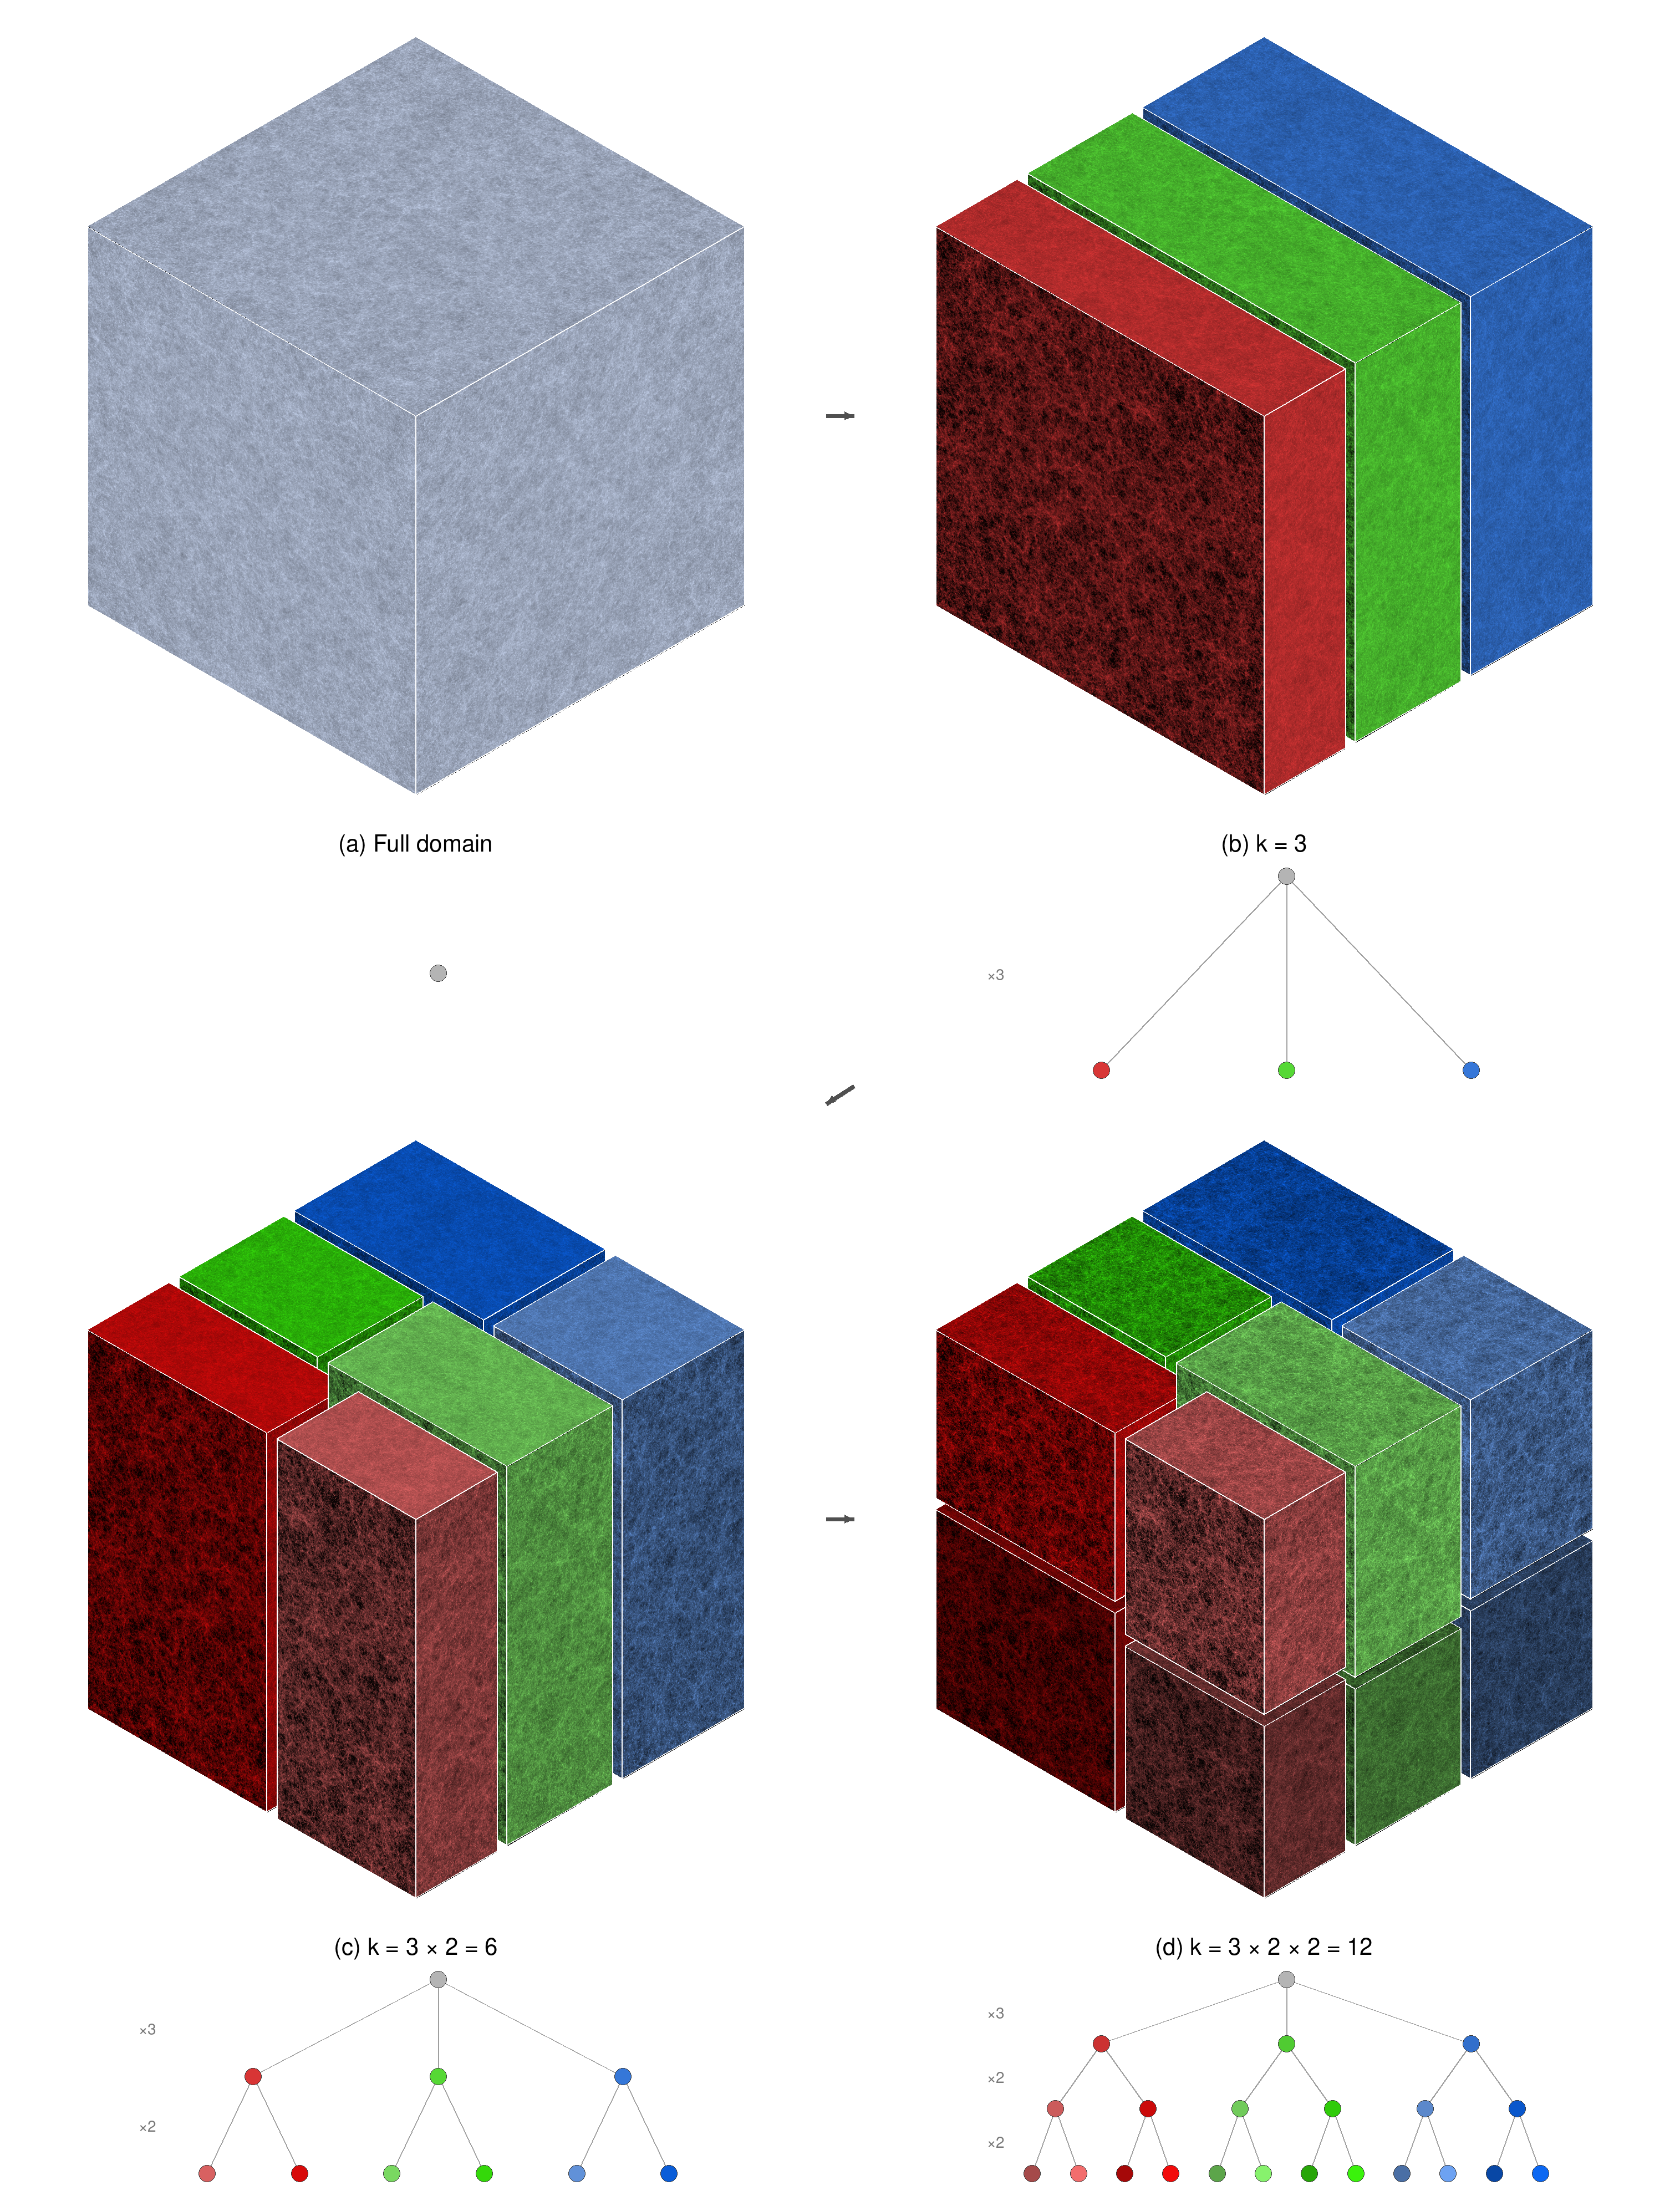
\includegraphics[width=\columnwidth]{../misc/ksection_progressive.png}
\caption{Progressive recursive \ksec\ decomposition for $\ncpu = 12 =
3 \times 2 \times 2$. (a)~The undivided simulation domain. (b)~First
split into $k = 3$ slabs along the longest axis. (c)~Each slab bisected
along the second axis ($3 \times 2 = 6$ sub-domains). (d)~Final bisection
along the third axis ($3 \times 2 \times 2 = 12$ leaf domains). Below
each panel, the corresponding \ksec\ tree is shown; colours encode
$x$-slab membership (red/green/blue), with saturation and brightness
indicating $y$ and $z$ subdivisions. Each face displays projected
column density from a $4096^3$ TSC density field. Sub-domain volumes
vary by ${\sim}10$--$30\,\%$, reflecting load-balanced wall placement.}
\label{fig:ksec_progressive}
\end{figure}

The tree is stored as a set of arrays indexed by node identifier.
For each internal node, the child indices for each of the $k_l$
partitions and the spatial coordinates of the partition boundaries
are recorded; for each leaf node, the assigned MPI rank is stored.
Every node also carries the minimum and maximum rank indices of all
leaves in its subtree, enabling rapid range queries during the
hierarchical exchange.

The total number of tree nodes,
$N_{\rm nodes} = 1 + \sum_{l=1}^{L} \prod_{i=1}^{l} k_i$,
is at most a few hundred for practical values of $\ncpu$
($\ncpu \leq 10^5$), representing negligible overhead.


\subsection{Load-Balanced Wall Placement}
\label{sec:ksec_loadbal}

When the tree is updated during load balancing (every \code{nremap}
coarse steps), the wall positions are adjusted by iterative
binary search so that each partition receives a load proportional to the
number of ranks it contains.

The procedure operates level by level, top to bottom. At level $l$:

\begin{enumerate}
\item A histogram is built over the splitting coordinate: for each
  node at level $l$, the cells within that node are projected onto the
  splitting axis and binned into a cumulative cost histogram with
  resolution $\Delta x_{\rm hist}$.

\item For each of the $k_l - 1$ walls within each node, a binary
  search adjusts the wall position until the cumulative
  load on the left side matches the target fraction. The target
  cumulative fraction for wall $j$ in a node spanning ranks
  $[i_{\rm min}, i_{\rm max}]$ with total count
  $n = i_{\rm max} - i_{\rm min} + 1$ is
  \begin{equation}
  f_j = n^{-1}\sum_{m=1}^{j} n_m,
  \label{eq:target_frac}
  \end{equation}
  where $n_m$ is the number of ranks assigned to partition $m$.
  Because $n$ ranks cannot always be divided evenly among $k_l$
  partitions, $n_m = \lfloor n/k_l \rfloor + 1$ for the first
  $n \bmod k_l$ partitions (which absorb the remainder), and
  $n_m = \lfloor n/k_l \rfloor$ for the rest.
  Here $\lfloor \cdot \rfloor$ denotes the floor function (the
  largest integer not exceeding the argument).

\item An \code{MPI\_ALLREDUCE} aggregates the local histograms across
  all $\ncpu$ ranks to obtain the global cumulative load at each wall
  position. The binary search converges when the relative load imbalance
  $|\hat{L}_j - L_j^{\rm target}| / L_j^{\rm target}$ falls below a
  tolerance $\epsilon_{\rm tol}$ (typically 1\,per\,cent), or when the
  wall position can no longer be resolved at the histogram resolution.

\item After wall convergence, the cells are repartitioned (sorted)
  according to the new wall positions, and the histogram bounds are
  updated for the next level.
\end{enumerate}


\subsection{Memory-Weighted Cost Function}
\label{sec:ksec_membal}

The default \ramses\ load balancer weights all cells equally.
\curamses\ supports an optional memory-weighted cost function:
\begin{equation}
C_{\rm cell} = 2^{-N_{\rm dim}}\bigl(w_{\rm grid} +
n_{\rm part}({\rm igrid}) \cdot w_{\rm part}\bigr),
\label{eq:cost_function}
\end{equation}
where $w_{\rm grid}$ is the memory cost per grid slot (default 270
bytes, accounting for hydro, gravity, and AMR bookkeeping arrays),
$w_{\rm part}$ is the memory cost per particle slot (default 12 bytes
for position, velocity, mass, and linked-list pointers), and
$n_{\rm part}({\rm igrid})$ is the number of particles attached to
grid \code{igrid}. The division by $\twotondim$ distributes the grid
cost evenly among its eight cells.

This cost function ensures that ranks hosting dense haloes (many
particles per cell) receive fewer cells, preventing memory exhaustion
on particle-heavy ranks. All histogram loads are accumulated in 64-bit
integers to avoid overflow when summing costs across millions of cells.

Activating memory-weighted balancing requires setting
\code{memory\_balance = .true.} and optionally tuning
\code{mem\_weight\_grid} and \code{mem\_weight\_part} in the namelist.
Our tests with $200\,\mathrm{M}$ particles on 12 ranks show that
memory-weighted balancing reduces the peak-to-mean memory ratio from
2.5 to 1.3 without affecting physics results (identical
$e_{\rm cons}$, $e_{\rm pot}$, $e_{\rm kin}$ to machine precision).

The parameter \code{nremap} controls the frequency of load-rebalancing
operations (every \code{nremap} coarse steps). We changed the default
from \code{nremap = 0} (rebalance every step) to \code{nremap = 5}
based on systematic tests with $200\,\mathrm{M}$ particles on 12 ranks over
10 coarse steps:

\begin{table}
\centering
\caption{Effect of \code{nremap} on total runtime and load-balance
overhead. All configurations produce identical physics results
($e_{\rm cons} = 3.77 \times 10^{-3}$ at step 10).}
\label{tab:nremap}
\begin{tabular}{cccc}
\toprule
\code{nremap} & Total (s) & LB time (s) & LB fraction \\
\midrule
1  & 303.8 & 64.4 & 21.2\% \\
3  & 269.9 & 24.7 &  9.1\% \\
5  & 249.8 & 15.7 &  6.3\% \\
10 & 258.6 & 11.6 &  4.5\% \\
\bottomrule
\end{tabular}
\end{table}

The optimal value \code{nremap = 5} balances the cost of rebalancing
against the growing imbalance that accumulates between rebalancing
steps. Higher values ($\code{nremap} = 10$) reduce LB overhead further
but allow imbalance to grow enough to slow other operations, resulting
in a net increase in total runtime.

To identify bottlenecks in the load-balancing procedure, we added
internal timing instrumentation that reports the wall-clock time of
each phase:
(i) \code{numbp\_sync} (MPI synchronization of particle counts for
virtual grids),
(ii) \code{cmp\_new\_cpu\_map} (histogram construction and wall
finding),
(iii) \code{expand\_pass} (ghost-zone expansion after grid migration),
(iv) \code{grid\_migration} (actual grid transfer between ranks),
(v) \code{allreduce+cpumap\_update} (global reduction and CPU map
reconstruction), and
(vi) \code{shrink\_pass} (removal of migrated grids from source rank).
Profiling reveals that \code{allreduce+cpumap\_update} dominates,
consuming approximately 50\,per\,cent of the total load-balance time.
This motivates the \code{nremap = 5} default, as reducing the
frequency of these expensive global operations has a disproportionate
impact on total runtime.


\section{HIERARCHICAL MPI COMMUNICATION}
\label{sec:ksec_exchange}

The tree structure described in Section~\ref{sec:ksec_tree} enables
a hierarchical exchange protocol that replaces the global
\code{MPI\_ALLTOALL} with a sequence of level-by-level correspondent
exchanges. We implement two variants.

\subsection{Exclusive Exchange}
\label{sec:ksec_exclusive}

In the exclusive exchange, each item
has a unique destination rank. The algorithm walks the \ksec\ tree
from root to leaf, where each \emph{node} represents a contiguous
group of MPI ranks at a given tree level. The \emph{root} node
encompasses all $\ncpu$ ranks and represents the entire computational
domain. At each level~$l$, a node is partitioned into $k_l$ child
nodes; the leaf nodes at the bottom of the tree correspond to
individual MPI ranks.  Algorithm~\ref{alg:exclusive} summarises the
procedure:

\begin{algorithm}[H]
\caption{Exclusive hierarchical exchange}
\label{alg:exclusive}
\begin{algorithmic}[1]
\REQUIRE Send buffer $\mathbf{S}$ with $N$ items, destination ranks $\mathbf{d}$
\ENSURE Receive buffer $\mathbf{R}$ with items destined for this rank
\STATE $\mathbf{W} \leftarrow \mathbf{S}$; $\mathbf{D} \leftarrow \mathbf{d}$; node $\leftarrow$ root
\FOR{$l = 1$ \TO $L$}
  \STATE $k \leftarrow k_l$; my\_child $\leftarrow$ \code{ksec\_cpu\_path}(myid, $l$)
  \STATE Classify items in $\mathbf{W}$ by child index (counting sort on $\mathbf{D}$)
  \STATE Identify $k-1$ correspondent ranks (one per sibling child)
  \FOR{each correspondent $p$}
    \STATE Exchange count: \code{MPI\_ISEND/IRECV} (tag $100+l$)
    \STATE Exchange data: \code{MPI\_ISEND/IRECV} (tags $200+l$, $300+l$)
  \ENDFOR
  \STATE \code{MPI\_WAITALL}
  \STATE $\mathbf{W} \leftarrow$ merge(my\_child items, received items)
  \STATE node $\leftarrow$ \code{ksec\_next}(node, my\_child)
\ENDFOR
\STATE $\mathbf{R} \leftarrow \mathbf{W}$
\end{algorithmic}
\end{algorithm}

At each level, each rank communicates with at most $k_l - 1$
correspondent ranks (one from each sibling subtree). The
correspondent in a sibling subtree of size $s$ is chosen as
$\min(\text{my\_pos}, s-1)$ to distribute load evenly. The total
number of messages per rank per exchange is
\begin{equation}
N_{\rm msg} = \sum_{l=1}^{L} (k_l - 1) = \sum_i m_i (p_i - 1),
\label{eq:msg_count}
\end{equation}
which for $\ncpu = 1024 = 2^{10}$ gives $N_{\rm msg} = 10$ --- two
orders of magnitude fewer than the ${\sim}1024$ messages required in
the original all-to-all pattern.

Figure~\ref{fig:hier_exchange} illustrates the communication pattern
for $\ncpu = 12\,(= 3 \times 2 \times 2)$. At level~1 ($k_1 = 3$),
the 12 ranks are grouped into three children of four ranks each. Each
rank exchanges data with one correspondent in each of the two sibling
subtrees, yielding $k_1 - 1 = 2$ communication steps: step~1 pairs
children~1 and~2 (e.g.\ rank~1 $\leftrightarrow$ rank~5), while
step~2 simultaneously pairs children~1 and~3 (dark red arcs,
e.g.\ rank~1 $\leftrightarrow$ rank~9) and children~2 and~3 (orange
arcs, e.g.\ rank~5 $\leftrightarrow$ rank~9). At level~2 ($k_2 = 2$),
the scope narrows to within each group of four, with each rank
contacting one correspondent two positions away (e.g.\ rank~1
$\leftrightarrow$ rank~3). Finally, at level~3 ($k_3 = 2$), only
adjacent pairs communicate (e.g.\ rank~1 $\leftrightarrow$ rank~2).
The progressively shorter arcs reflect the hierarchical narrowing of
communication scope: long-range inter-group exchanges are resolved
first, and successive levels refine the routing within ever-smaller
subtrees. Each rank sends a total of $N_{\rm msg} = 2 + 1 + 1 = 4$
messages per exchange, independent of $\ncpu$.

The pairing structure at each tree level follows directly from the
branching factor. When a node has $p$ children, data from every child
must reach every other child. This is accomplished in $p - 1$
sequential steps. In step~$s$ ($s = 1, \ldots, p-1$), child~$s+1$ is
paired with each of the children $1, \ldots, s$: each rank in
child~$s+1$ exchanges data with its correspondent in child~$c$ for
$c = 1, \ldots, s$, yielding $s$ concurrent point-to-point exchanges.
After step~$s$, every child $1$ through $s+1$ holds the aggregate of
all data originating from children $1$ through $s+1$. In particular,
after all $p - 1$ steps, every child possesses the complete data set
of the entire subtree. For the $\ncpu = 12$ example in
Figure~\ref{fig:hier_exchange}, level~1 has $k_1 = 3$, giving
$3 - 1 = 2$ steps: step~1 pairs child~2 with child~1 ($1 \times 4$
exchanges), and step~2 pairs child~3 with both children~1 and~2
($2 \times 4$ exchanges). Levels~2 and~3 each have $k = 2$, requiring
only $2 - 1 = 1$ step per level.

A trade-off of the hierarchical routing is that the total data volume
transmitted per rank exceeds that of a direct \code{MPI\_ALLTOALL}.
In the all-to-all pattern, each rank sends each item exactly once to
its destination. In the hierarchical exchange, an item may be
forwarded through multiple tree levels before reaching its final
destination, so the same data can traverse several hops. In the worst
case, a rank's entire send buffer is relayed at every level,
giving a per-rank volume of at most $L \times V_{\rm local}$, where
$V_{\rm local}$ is the rank's data size. However, this upper bound is
rarely approached in practice because items are filtered by child
index at each level: only the subset destined for a sibling subtree
is actually transmitted, and successive levels operate on
progressively smaller subsets. The key advantage, reducing the number
of communication partners from $\Olog{\ncpu}$ to $\Olog{\sum_l k_l}$,
more than compensates for the modest increase in aggregate volume,
particularly at large $\ncpu$ where message startup latency dominates.

\begin{figure}
\centering
\includegraphics[width=\columnwidth]{../misc/hierarchical_exchange.pdf}
\caption{Hierarchical exchange communication pattern for $\ncpu = 12
\,(= 3 \times 2 \times 2)$. Coloured rectangles represent MPI ranks
numbered 1--12, using the same colour scheme as
Figure~\ref{fig:ksec_progressive}. Arcs denote bidirectional
point-to-point exchanges.  At level~1 ($k_1 = 3$), two steps connect
each rank with correspondents in the two sibling subtrees; the
two colours in step~2 distinguish the children~1$\leftrightarrow$3
(dark red) and children~2$\leftrightarrow$3 (orange) pairings that
proceed concurrently.  At levels~2 and~3 ($k_2 = k_3 = 2$), the
communication range contracts to within each group and then to
adjacent pairs.  The total message count per rank is
$N_{\rm msg} = (3{-}1) + (2{-}1) + (2{-}1) = 4$.}
\label{fig:hier_exchange}
\end{figure}

Working buffers are managed with Fortran 2003 \code{move\_alloc} for
zero-copy buffer swaps at each level, and per-level arrays (child
counts, peer lists, MPI request handles) are pre-allocated with
\code{save} attributes to eliminate allocation/deallocation overhead
on repeated calls.


\subsection{Ghost-Zone Exchange via K-Section}
\label{sec:ksec_ghostzone}

The ghost-zone (virtual boundary) exchange is the most
communication-intensive operation in \ramses, called multiple times per
fine time step for hydro, gravity, and particle updates. We replace
the standard all-to-all pattern with four \ksec-based variants.
First, a forward exchange sends data from emission grids to reception
grids, and a corresponding reverse accumulation adds received values
back into the emission grids. Because the hierarchical routing
internally uses double-precision buffers, an integer variant packs
integer data (e.g.\ \code{cpu\_map}, \code{flag1}) into
double-precision words before transport and unpacks them on receipt,
reusing the same tree-walk machinery without a separate integer
communication path.

The data packing format for each ghost grid is:
\begin{equation}
\text{sendbuf}(1:\twotondim+2,\, i) = \bigl\{
u_1, \ldots, u_{\twotondim},\, \text{sender\_id},\, \text{index}
\bigr\},
\label{eq:sendbuf_format}
\end{equation}
where $u_j$ are the cell data values, \code{sender\_id} identifies the
source rank, and \code{index} is the emission or reception array index
used for scatter at the receiver. This self-describing format enables
the receiver to place incoming data without maintaining separate
communication tables.


For multi-variable exchanges (e.g.\ all hydro conserved variables), we
provide bulk variants that pack all $N_{\rm var}$ columns of a 2D
array into a single \ksec\ exchange call:
\begin{equation}
\text{sendbuf}\bigl((v-1)\twotondim + j,\, i\bigr) =
\text{xx}(v,\, \text{cell}_{i,j}),
\label{eq:bulk_format}
\end{equation}
for $v = 1, \ldots, N_{\rm var}$ and $j = 1, \ldots, \twotondim$,
plus two metadata entries. This amortises the tree-walk overhead and
MPI latency over $N_{\rm var}$ variables, yielding a significant
reduction in the number of exchange calls per time step (from
$N_{\rm var}$ individual calls to a single bulk call at each of the
five call sites in \code{amr\_step}).


\subsection{Communication Structure Construction}
\label{sec:ksec_buildcomm}

The construction of the communication structure, which determines
which grids must be exchanged as ghost zones, was itself based on
\code{MPI\_ALLTOALL} in the original \ramses. We replace this with a
\ksec\ exchange: each rank packs its reception grids as triplets
(sender identifier, reception index, grid address), sends them via
the exclusive hierarchical exchange, and the receiver reconstructs
its emission arrays from the incoming data. This eliminates the last
remaining all-to-all communication pattern in the AMR infrastructure.

The \ksec\ exchange routines and virtual boundary functions contain
numerous small arrays (child counts, peer lists, MPI request handles,
receive buffers) that are allocated and deallocated on every call. At
100+ calls per time step, the cumulative allocation overhead becomes
non-negligible. We convert these to \code{save} variables with
grow-only semantics: the buffer is allocated on first use and grown
(but never shrunk) when a larger size is needed. The receive buffer's
first dimension must match the \code{nprops} parameter exactly (for
correct MPI stride), so reallocation is triggered when either the
capacity or the property count changes. This optimization eliminates
approximately 100 allocation/deallocation pairs per exchange call.


\subsection{Complexity Analysis}
\label{sec:ksec_complexity}

Table~\ref{tab:complexity} summarizes the communication complexity of
the original \ramses\ and \curamses.

\begin{table}
\centering
\caption{Communication complexity per ghost-zone exchange operation.
$N_{\rm ghost}$ is the total number of ghost grids per rank; $k_l$
are the branching factors at tree level $l$.}
\label{tab:complexity}
\begin{tabular}{lcc}
\toprule
& Original \ramses & \curamses \\
\midrule
Message count & $\Olog{\ncpu}$ & $\Olog{\sum_l k_l}$ \\
Buffer memory & $\Olog{\ncpu \cdot N_{\rm ghost}}$ &
  $\Olog{k_{\rm max} \cdot N_{\rm ghost}}$ \\
\code{MPI\_ALLTOALL} calls & $\geq 1$ per exchange & 0 \\
\bottomrule
\end{tabular}
\end{table}


% ===================================================================
% 4. MORTON KEY HASH TABLE AND MEMORY OPTIMIZATIONS
% ===================================================================
\section{MORTON KEY HASH TABLE AND MEMORY OPTIMIZATIONS}
\label{sec:morton}

\subsection{The Nbor Array Problem}
\label{sec:morton_problem}

\ramses\ stores the octree connectivity in several arrays, the largest
of which is \code{nbor(1:ngridmax, 1:twondim)} --- a six-column
integer array that records, for each grid, the cell index of its
neighbour in each of the six Cartesian directions ($\pm x$, $\pm y$,
$\pm z$). Each entry is a 64-bit integer occupying 8\,bytes, so this
array consumes $48\,\ngridmax$ bytes --- 240\,MB for
$\ngridmax = 5\,\mathrm{M}$.
Moreover, the \code{nbor} array must be maintained during grid creation,
deletion, defragmentation, and inter-rank migration --- a significant
source of code complexity and a potential source of bugs.


\subsection{Morton Key Encoding and Neighbour Arithmetic}
\label{sec:morton_encoding}

A Morton key (also known as a Z-order key) is a 64-bit integer formed
by interleaving the bits of the three-dimensional integer coordinates
$(i_x, i_y, i_z)$ of a grid at its AMR level:
\begin{equation}
M(i_x, i_y, i_z) = \sum_{b=0}^{B-1}
\Bigl[
  \text{bit}_b(i_x) \cdot 2^{3b} +
  \text{bit}_b(i_y) \cdot 2^{3b+1} +
  \text{bit}_b(i_z) \cdot 2^{3b+2}
\Bigr],
\label{eq:morton_encode}
\end{equation}
where $B = 21$ bits per coordinate and $\text{bit}_b(n)$
extracts bit $b$ of integer $n$. Here $n_x$ denotes the number of
coarse-level grid cells per dimension (a \ramses\ parameter, typically
1--4). At AMR level $l$, there are $n_x \cdot 2^{l-1}$ grid cells
per dimension, so the integer coordinate range is $[0,\, n_x \cdot
2^{l-1})$. With $B = 21$ bits the maximum representable coordinate is
$2^{21} - 1 = 2\,097\,151$, which accommodates up to level 22 for
$n_x = 1$ or level 20 for $n_x = 4$. The encoding and decoding
(the inverse map $(i_x, i_y, i_z) = M^{-1}(\text{key})$) are
implemented with simple bit-shift loops.

The integer coordinates of a grid at level $l$ are computed from its
floating-point centre position $\mathbf{x}_g$ as
\begin{equation}
i_d = \lfloor x_{g,d} \cdot 2^{l-1} \rfloor, \quad d \in \{x, y, z\},
\label{eq:grid_to_int}
\end{equation}
where $\lfloor \cdot \rfloor$ denotes the floor function and
coordinates are in units of the coarse grid spacing.
Note that AMR does not populate all possible grid positions at a given
level: only regions that satisfy the refinement criteria contain grids.
The Morton key therefore serves as a unique spatial address for each
\emph{existing} grid; the hash table (Section~\ref{sec:morton_hashtable})
stores only the grids that are actually allocated, making the
look-up cost independent of the total number of potential grid
positions at that level.

The neighbour of a grid in direction $j$ (using the \ramses\ convention
$1 = -x$, $2 = +x$, $3 = -y$, $4 = +y$, $5 = -z$, $6 = +z$) is
obtained by:
(i) decoding the Morton key via the inverse map
  $(i_x, i_y, i_z) = M^{-1}(\text{key})$;
(ii) incrementing or decrementing the appropriate coordinate;
(iii) applying periodic wrapping if the coordinate exceeds
  $[0, n_d \cdot 2^{l-1})$;
(iv) re-encoding to obtain the neighbour's Morton key.
The parent key is obtained by a 3-bit right shift: $M_{\rm parent} =
M \gg 3$. A child key is obtained by a 3-bit left shift plus the
child index (0--7): $M_{\rm child} = (M \ll 3) \,|\, i_{\rm child}$.


\subsection{Per-Level Hash Table and Replacement Functions}
\label{sec:morton_hashtable}

We maintain one open-addressing hash table (probing consecutive slots
on collision) per AMR level, mapping Morton keys $M$ to grid indices
\code{igrid}.

The hash function uses multiplicative hashing
with an additional mixing step:
\begin{equation}
h(M) = \bigl[\bigl((M \times \phi_1) \oplus (M \gg 16)\bigr) \times
\phi_2\bigr] \oplus (h \gg 13),
\label{eq:hash_func}
\end{equation}
where $\phi_1 = 2654435761$ and $\phi_2 = \texttt{0x9E3779B97F4A7C15}$
are constants chosen for good bit mixing, and the table capacity is
always a power of two to allow bitmask modular arithmetic. Collisions
are resolved by linear probing; the load factor is kept below 0.7 by
automatic rehashing (doubling capacity).

The hash table is maintained incrementally:
\begin{itemize}
\item \code{morton\_hash\_insert}: called during \code{make\_grid\_coarse} and \code{make\_grid\_fine};
\item \code{morton\_hash\_delete}: called during \code{kill\_grid};
\item Full rebuild after defragmentation (\code{morton\_hash\_rebuild}).
\end{itemize}

A companion array \code{grid\_level(igrid)} stores the AMR level of
each grid, enabling Morton key computation from the grid index alone.

Two wrapper functions provide drop-in replacements for the original
\code{nbor}-based access patterns:

\begin{itemize}
\item \code{morton\_nbor\_grid(igrid, ilevel, j)}: returns the grid
  index of the same-level neighbour in direction $j$, replacing the
  pattern \code{son(nbor(igrid, j))}. Implemented as: compute Morton
  key, shift by direction, look up in hash table.

\item \code{morton\_nbor\_cell(igrid, ilevel, j)}: returns the father
  cell index of the neighbour, replacing the pattern
  \code{nbor(igrid, j)}. For level 1, returns the coarse cell index
  directly; for finer levels, computes the parent grid via the
  hash table at level $l-1$ and the octant index from the coordinate
  parity.
\end{itemize}

The \code{nbor} array is reduced to \code{allocate(nbor(1:1, 1:1))}
--- effectively eliminated while maintaining compilation compatibility
with any remaining references.

\begin{figure*}
\centering
\includegraphics[width=\textwidth]{fig_morton_hash.pdf}
\caption{Schematic of the Morton key hash table that replaces the
  original \code{nbor} array.  Left: the eliminated
  \code{nbor($\ngridmax$, 6)} array (240\,MB for $\ngridmax = 5$\,M).
  Right: the replacement workflow --- grid cell coordinates
  $(i_x, i_y, i_z)$ are bit-interleaved into a 64-bit Morton key $M$,
  which is mapped to a grid index \code{igrid} via a per-level
  open-addressing hash table with multiplicative hashing.  The hash
  table memory footprint is $\approx 17\,N_{\rm grids}$ bytes
  (typically $<$50\,MB), yielding a net saving of $>$190\,MB per rank.}
\label{fig:morton_hash}
\end{figure*}

\subsection{Hilbert Key and Histogram Array Elimination}
\label{sec:mem_hilbert}

When using \ksec\ ordering, the Hilbert key array
\code{hilbert\_key(1:ncell)} is no longer needed for domain
decomposition. We replace it with \code{allocate(hilbert\_key(1:1))},
saving $16 \times \ngridmax \times \twotondim$ bytes
under \code{QUADHILBERT} (128-bit keys stored as two 64-bit integers).
For $\ngridmax = 5\,\mathrm{M}$, this is approximately 640\,MB.

The defragmentation routine, which previously required Hilbert keys
for reordering, uses a local scratch array (\code{defrag\_dp})
allocated only during the defragmentation pass and immediately
deallocated.

Similarly, the arrays \code{bisec\_ind\_cell} and \code{cell\_level},
each of size $\ngridmax \times \twotondim$ integers (8 bytes), are used
exclusively during load balancing to build the bisection histogram.
We allocate them on entry to \code{init\_bisection\_histogram} and
deallocate them after \code{cmp\_new\_cpu\_map} returns, saving
$2 \times 8 \times \ngridmax \times \twotondim \approx 320$\,MB
for $\ngridmax = 5\,\mathrm{M}$. Since load balancing occurs only
every \code{nremap} coarse steps, these arrays are absent during the
vast majority of the simulation.


\subsection{Memory Savings Summary}
\label{sec:mem_summary}

The memory cost of the hash table is
\begin{equation}
M_{\rm hash} \approx \frac{N_{\rm grids}}{0.7} \times
(8 + 4) \text{ bytes} \approx 17\,N_{\rm grids} \text{ bytes},
\label{eq:hash_memory}
\end{equation}
where $N_{\rm grids}$ is the actual number of grids (typically much
less than $\ngridmax$), 8 bytes per key, 4 bytes per grid index, and
a load factor of 0.7 accounts for empty slots. The
\code{grid\_level} array adds $4 \times \ngridmax$ bytes.

Compared to the original \code{nbor} cost of $48 \times \ngridmax$
bytes, the net savings are approximately
$44\,\ngridmax - 17\,N_{\rm grids}$.
Since $N_{\rm grids} \ll \ngridmax$ in practice (typical occupancy is
30--60\,per\,cent), the savings are substantial: $\sim$176\,MB for
$\ngridmax = 5\,\mathrm{M}$ at 50\,per\,cent occupancy.

The computational cost of a hash lookup is $\Olog{1}$ expected time,
with worst-case linear probing bounded by the load factor. In
practice, the precomputed neighbour caches described in
Section~\ref{sec:multigrid} amortize any per-lookup overhead in the
performance-critical Poisson solver.

Table~\ref{tab:memory} summarizes the combined memory savings for
$\ngridmax = 5\,\mathrm{M}$.

\begin{table}
\centering
\caption{Memory savings per MPI rank for $\ngridmax = 5\,\mathrm{M}$.
Savings marked with ${}^*$ are conditional on using \ksec\ ordering.}
\label{tab:memory}
\small
\begin{tabular}{lrl}
\toprule
Optimization & MB & Availability \\
\midrule
\code{nbor} removal (Morton hash) & 240 & Always \\
\code{hilbert\_key} removal${}^*$ & 640 & Steady state \\
On-demand \code{bisec\_ind\_cell}${}^*$ & 160 & Between LB \\
On-demand \code{cell\_level}${}^*$ & 160 & Between LB \\
Defrag scratch (local) & 40 & Between defrag \\
\midrule
\textbf{Total} & \textbf{$>$1200} & \\
\bottomrule
\end{tabular}
\end{table}

The reported memory savings of the \code{nbor} array account for both
the eliminated array ($48\,\ngridmax = 240$\,MB) and the hash table
overhead ($\sim$17\,$N_{\rm grids}$, typically $<$50\,MB). Net savings
are at least 190\,MB. The Hilbert key savings of 640\,MB assume
\code{QUADHILBERT}; for standard 64-bit keys the savings would be
320\,MB. Figure~\ref{fig:memory_savings} visualizes the individual
contributions.

\begin{figure*}
\centering
\includegraphics[width=\textwidth]{fig_memory_savings.pdf}
\caption{Per-rank memory savings breakdown for $\ngridmax = 5$\,M.
  Solid bars denote unconditional savings (always available); hatched
  bars denote savings available only between load-balance steps or
  defragmentation passes.  The red segment shows the hash table
  overhead ($\sim$40--50\,MB), yielding a net saving of $>$1190\,MB
  per MPI rank.}
\label{fig:memory_savings}
\end{figure*}

We implement a diagnostic routine \code{writemem\_minmax} that reports
the minimum and maximum resident set size across all ranks at each
coarse step, providing runtime verification of the memory savings.


% ===================================================================
% 5. MULTIGRID SOLVER OPTIMIZATIONS
% ===================================================================
\section{MULTIGRID POISSON SOLVER OPTIMIZATIONS}
\label{sec:multigrid}

The multigrid (MG) Poisson solver consumes a large fraction of the
total runtime in self-gravitating cosmological simulations. In
baseline \ramses, profiling reveals that the MG solver accounts for
approximately 55\,per\,cent of the total wall-clock time per coarse
step. We describe several optimizations that reduce this fraction to
approximately 39\,per\,cent.


\subsection{Neighbour Grid Precomputation}
\label{sec:mg_nbor_precompute}

The Gauss--Seidel (GS) smoother and residual computation both require
access to the six Cartesian neighbours of each grid. In the Morton
hash table approach (Section~\ref{sec:morton}), each neighbour lookup
involves a hash table query. While individual lookups are $\Olog{1}$,
the GS kernel accesses 6 neighbours per grid, 8 cells per grid, and
typically 4--5 V-cycle iterations, resulting in hundreds of hash
lookups per grid per solve.

We precompute all neighbour grids into a contiguous array before
entering the V-cycle iteration loop:
\begin{equation}
\text{nbor\_grid\_fine}(j,\, i) = \text{morton\_nbor\_grid}(
\text{igrid\_amr}(i),\, l,\, j),
\label{eq:nbor_precompute}
\end{equation}
for $j = 0, 1, \ldots, 6$ (where $j = 0$ stores the grid's own AMR
index \code{igrid\_amr}) and $i = 1, \ldots, N_{\rm grid}$. This
array is allocated before the iteration loop and deallocated after,
so its memory overhead is transient.

The original GS kernel also contains a branch on \code{igshift == 0}
to distinguish between the current grid and its neighbours. We unify
the access pattern with a cache array
\code{nbor\_grids\_cache(0:twondim)}, where index 0 references the
grid itself. All neighbour accesses --- including the self-reference ---
use the same indexed load, eliminating the branch.


\subsection{Merged Red-Black Exchange and Fused Kernels}
\label{sec:mg_merged_rb}

Standard red-black Gauss--Seidel smoothing in \ramses\ performs a
ghost-zone exchange of the potential $\phi$ between the red and black
sweeps:
Red $\to$ Exchange($\phi$) $\to$ Black $\to$ Exchange($\phi$).
Each iteration thus requires two exchanges for the smoother alone,
plus additional exchanges for the residual and restriction/prolongation
steps --- a total of 9 exchange calls per iteration.

We merge the red and black sweeps by removing the inter-sweep exchange:
Red $\to$ Black $\to$ Exchange($\phi$).
This is a form of relaxed synchronisation: boundary cells in the
black sweep use values from the previous iteration rather than
freshly exchanged red-sweep values. For the MG
preconditioner, this does not affect convergence in practice --- the
MG solve is itself an approximate preconditioner for the conjugate
gradient outer iteration, and the stale-ghost error is well within
the MG tolerance.

We also remove two unnecessary residual exchanges per iteration,
reducing the total from 9 to 5 exchange calls per iteration --- a
44\,per\,cent reduction in MG communication volume.

The same optimization is applied to the coarse-level solver
(direct solve, pre-smoothing, post-smoothing), where the merged
red-black pattern similarly halves the exchange count.

The MG algorithm requires both the residual $r = f - A\phi$ and its
$L^2$ norm $\|r\|_2^2$ at specific points in the V-cycle. In the
original code, these are computed in separate passes. We add an
optional \code{norm2} argument to \code{cmp\_residual\_mg\_fine}:
when present, the norm is accumulated during the same loop that
computes the residual, saving one full grid traversal.
Since the subroutine is \code{external} (not module-contained), callers
must include an \code{interface} block to enable the optional-argument
dispatch.

The GS fast-path computation involves a division by
$2 N_{\rm dim} = 6$:
\begin{equation}
\phi_{\rm new} = \frac{\sum_j \phi_j - h^2 f}{2 N_{\rm dim}}.
\label{eq:gs_update}
\end{equation}
We replace the division \code{/ dtwondim} with a multiplication by
the precomputed reciprocal \code{* oneoverdtwondim}, which is faster
on most architectures.

\begin{figure*}
\centering
\includegraphics[width=\textwidth]{fig_mg_redblack.pdf}
\caption{Multigrid V-cycle exchange optimization.
  (a)~Original: each smoothing iteration requires 9 ghost-zone
  exchanges --- two for the red-black sweeps (exchanging $\phi$), one
  each for the residual and norm (exchanging $r$), and additional
  exchanges for restriction and prolongation.
  (b)~Optimized: the inter-sweep red-black exchange is removed
  (relaxed synchronisation), and the separate residual and norm
  exchanges are fused, reducing the total to 5 exchanges per iteration
  ($-44$\,per\,cent).  Orange diamonds marked ``E'' denote active
  exchanges; crossed-out diamonds indicate eliminated exchanges.}
\label{fig:mg_redblack}
\end{figure*}

\subsection{Performance Impact}
\label{sec:mg_performance}

Combining all optimizations, the MG Poisson solver's share of total
runtime is reduced from 55.1\,per\,cent to 38.6\,per\,cent in a
representative test ($200\,\mathrm{M}$ particles, 12 ranks, 10 coarse
steps). The iteration counts are unchanged (Level~8: 5 iterations,
Level~9: 4 iterations), confirming that the merged red-black exchange
does not degrade convergence.


% ===================================================================
% 6. FEEDBACK SPATIAL BINNING
% ===================================================================
\section{FEEDBACK SPATIAL BINNING}
\label{sec:feedback}

\subsection{The Brute-Force Bottleneck}
\label{sec:fb_problem}

The Type~II supernova (SNII) feedback implementation in \ramses\
involves two computationally expensive routines:

\begin{itemize}
\item \code{average\_SN}: averages hydrodynamic quantities within the
  blast radius of each SN event, accumulating volume, momentum, kinetic
  energy, mass loading, and metal loading. The original implementation
  loops over all cells $\times$ all SNe, yielding
  $\Olog{N_{\rm cells} \times N_{\rm SN}}$ complexity.

\item \code{Sedov\_blast}: injects the blast energy and ejecta into
  cells within the blast radius. Same $\Olog{N_{\rm cells} \times
  N_{\rm SN}}$ complexity.
\end{itemize}

In production simulations with $\sim$2000 simultaneous SN events,
these routines consume 66\,s and 11\,s per call respectively,
dominating the feedback time step.


\subsection{Spatial Hash Binning}
\label{sec:fb_binning}

We partition the simulation domain into a uniform grid of
$n_{\rm bin}^3$ bins, where
$n_{\rm bin} = \max(1,\, \min(128,\, \lfloor L_{\rm box} /
r_{\rm max} \rfloor))$
and $r_{\rm max}$ is the maximum SN blast radius (the larger of
\code{rcell} $\times$ \code{dx\_min} and \code{rbubble}). Each SN
event is assigned to a bin based on its position, and a linked list
threads the events within each bin:
$\text{bin\_head}(i_x, i_y, i_z) \to \text{SN}_1 \to
\text{SN}_2 \to \cdots$

For each cell, we compute its bin index and check only the 27
neighbouring bins (the cell's own bin plus its 26 face-, edge-, and
corner-adjacent bins). Since $r_{\rm max}$ is at most the bin size by
construction, this 27-bin neighbourhood is guaranteed to contain all
SNe that could influence the cell. The complexity becomes
$\Olog{N_{\rm cells} \times \bar{n}_{\rm SN/bin} \times 27}$,
where $\bar{n}_{\rm SN/bin} = N_{\rm SN} / n_{\rm bin}^3$ is the
average number of SNe per bin. Figure~\ref{fig:spatial_binning}
contrasts the two approaches.

\begin{figure*}
\centering
\includegraphics[width=\textwidth]{fig_spatial_binning.pdf}
\caption{Feedback spatial binning concept (shown in 2D for clarity).
  (a)~Brute force: every cell (blue square) must check all SN events
  (orange stars), resulting in $\Olog{N_{\rm cells} \times N_{\rm SN}}$
  complexity.
  (b)~Spatial hash binning: the domain is partitioned into a uniform
  grid of bins.  Each cell checks only the 27 neighbouring bins (9 in
  2D), shown as shaded regions, reducing the complexity to
  $\Olog{N_{\rm cells} \times 27\,\bar{n}_{\rm SN/bin}}$.  Distant SN
  events (grey) are never examined.}
\label{fig:spatial_binning}
\end{figure*}

\subsection{Performance Results}
\label{sec:fb_performance}

The binned \code{average\_SN} uses cell-parallel OpenMP threading:
the outer loop is over grids (with \code{!\$omp parallel do}), and
each thread processes the cells of one grid. When a cell falls within
an SN blast radius, the thread accumulates its contribution using
\code{!\$omp atomic} directives on the shared SN-indexed arrays
(\code{vol\_gas}, \code{dq}, \code{ekBlast}, etc.). The atomic
overhead is minimal because collisions are rare --- most bins contain
zero or one SN, so contention is low.
The \code{Sedov\_blast} routine writes only to cells owned by each
grid, so no atomics are needed. The outer loop is over grids, and
each thread independently processes the cells of its assigned grids,
checking only the 27 neighbouring bins for relevant SNe.

With approximately 2000 simultaneous SN events:
\begin{itemize}
\item \code{average\_SN}: 66\,s $\rightarrow$ 0.25\,s
  ($\sim$260$\times$ speedup)
\item \code{Sedov\_blast}: 11\,s $\rightarrow$ 0.07\,s
  ($\sim$157$\times$ speedup)
\end{itemize}

Verification by restarting at the same snapshot confirms bit-identical
results for all conservation quantities ($m_{\rm cons}$,
$e_{\rm cons}$, $e_{\rm pot}$, $e_{\rm kin}$, $e_{\rm int}$).

The same spatial binning technique is applied to the AGN feedback
routines (\code{average\_AGN} and \code{AGN\_blast}), which suffer
from the same $\Olog{N_{\rm cells} \times N_{\rm AGN}}$ brute-force
scaling. In production simulations with tens of thousands of active
AGN sink particles, these routines dominate the sink-particle time
step.

The AGN feedback involves three distinct interaction modes (saved
energy injection, jet feedback, and thermal feedback), each with a
different geometric distance criterion. The spatial binning is
agnostic to these distinctions: it reduces the candidate AGN set from
the full population to only those in the 27 neighbouring bins, while
preserving all distance-check logic and physical calculations
unchanged. The linked-list construction and 27-bin traversal follow
the same pattern as the SNII implementation
(\S\ref{sec:fb_binning}), with \code{bin\_head} and \code{agn\_next}
arrays replacing the SN-specific versions.

With approximately 32\,000 active AGN particles, the binned
\code{average\_AGN} achieves a $30\times$ speedup and \code{AGN\_blast}
a $14\times$ speedup, reducing the total AGN feedback time by a factor
of $\sim$4. Verification confirms bit-identical conservation
diagnostics compared to the original brute-force implementation.


% ===================================================================
% 7. VARIABLE-NCPU RESTART
% ===================================================================
\section{VARIABLE-NCPU RESTART}
\label{sec:varcpu}

\subsection{HDF5 Parallel I/O and Restart}
\label{sec:hdf5}

Standard \ramses\ writes one binary file per MPI rank per output.
Restarting with a different number of ranks is not directly supported,
requiring an intermediate step of reading with the original rank count,
redistributing, and re-writing.

We implement HDF5 parallel I/O using the HDF5 library's MPI-IO
backend. All ranks write to (and read from) a single HDF5 file,
with datasets organized hierarchically:
\begin{itemize}
\item \code{/amr/level\_\{l\}/}: grid positions, son flags, CPU map
  for each AMR level.
\item \code{/hydro/level\_\{l\}/}: conserved variables $\rho$,
  $\rho\mathbf{v}$, $E$, etc.
\item \code{/gravity/level\_\{l\}/}: gravitational potential $\phi$
  and force components.
\item \code{/particles/}: positions, velocities, masses, IDs, levels,
  formation times, metallicities.
\item \code{/sinks/}: sink particle properties.
\end{itemize}

When the number of ranks in the output file ($\ncpu^{\rm file}$)
differs from the current run ($\ncpu$), the following procedure
executes during restart:

\begin{enumerate}
\item Build a uniform \ksec\ tree for the new $\ncpu$ (equal-volume
  partitioning, without load-balance adjustment).
\item Read all grids from the HDF5 file. Since the file is a single
  shared file, all ranks can access all data.
\item For each grid, compute the CPU ownership from the father cell's
  position using \code{cmp\_ksection\_cpumap}.
\item Each rank retains only the grids assigned to it, building the
  local AMR tree incrementally.
\item Hydro, gravity, and particle data are read and scattered to
  locally owned grids using a precomputed file-index-to-local-grid
  mapping (\code{varcpu\_grid\_file\_idx}).
\item On the first coarse step after restart, a forced load-balance
  operation redistributes grids for optimal balance under the new rank
  configuration.
\end{enumerate}

This approach requires that all ranks temporarily hold the full grid
metadata (positions and son flags) during the reconstruction phase.
For typical production outputs (${\sim}10\,\mathrm{M}$ total grids), this
temporary overhead is a few hundred MB --- well within the memory
budget freed by the optimizations of Section~\ref{sec:morton}.


\subsection{Binary Distributed I/O Restart}
\label{sec:varcpu_binary}

When HDF5 is unavailable or the native binary format
(\code{informat='origin'}) is preferred, a distributed I/O strategy
enables variable-$\ncpu$ restart from the per-rank binary files
written by standard \ramses.  The binary format stores one file per
MPI rank --- \code{amr\_XXXXX.outYYYYY},
\code{hydro\_XXXXX.outYYYYY}, etc. --- so the number of files equals
$\ncpu^{\rm file}$, which may differ from the current $\ncpu$.

The restart proceeds in three stages.

\paragraph{Stage 1: Early detection and file assignment.}
Rank~1 probes the header of file~00001 to read $\ncpu^{\rm file}$.
If $\ncpu^{\rm file} \ne \ncpu$, the variable-$\ncpu$ path is
activated (requiring \ksec\ ordering).  The $\ncpu^{\rm file}$ files
are distributed among the $\ncpu$ ranks by round-robin assignment:
rank $r$ reads files whose index satisfies
$(f - 1) \bmod \ncpu = r - 1$.

\paragraph{Stage 2: Distributed AMR reconstruction.}
Each rank reads only its assigned AMR files, extracting per-level
active grid metadata (positions $\mathbf{x}_g$ and son flags).  The
per-level active grid counts are aggregated via
\code{MPI\_ALLREDUCE}.  For each level, the grids read by each rank
are assigned to their correct owner by evaluating
\code{cmp\_ksection\_cpumap} on the father cell position (computed
from $\mathbf{x}_g$ and the parent--child octant relationship).
An \code{MPI\_ALLTOALLV} exchange then routes each grid's data to
its owner, who creates the local AMR grid.  The exchange metadata
--- send ordering and receive-grid mapping --- is stored for reuse.

\paragraph{Stage 3: Hydro and gravity scatter.}
The hydro and gravity binary files are read in the same distributed
fashion: each rank reads only its assigned files and packs the
cell-centred data into per-level send buffers using the stored
send ordering.  The same \code{MPI\_ALLTOALLV} counts and
displacements from Stage~2 are reused, and the receive-grid mapping
scatters incoming data to the correct local cells.  Since the binary
format stores primitive variables (density, velocity, pressure),
a primitive-to-conservative conversion is applied on the receiving
side.

Particle files are handled independently: each rank reads its
assigned files and retains only those particles whose positions fall
within the local \ksec\ domain.

This three-stage approach ensures that no rank reads more than
$\lceil \ncpu^{\rm file} / \ncpu \rceil$ files (at most two for
practical configurations), and the \code{MPI\_ALLTOALLV} exchange
per level has cost proportional to the number of grids exchanged
rather than the total number of ranks.  Verification tests confirm
$e_{\rm cons} = 0$ for both upward ($4 \to 12$) and downward
($12 \to 4$) rank-count changes.
Figure~\ref{fig:varcpu_flow} summarizes the three-stage pipeline.

\begin{figure*}
\centering
\includegraphics[width=\textwidth]{fig_varcpu_flow.pdf}
\caption{Three-stage distributed I/O pipeline for binary
  variable-$\ncpu$ restart.
  Stage~1 (blue): the header is probed to detect a rank-count mismatch,
  and the $\ncpu^{\rm file}$ files are assigned to $\ncpu$ ranks by
  round-robin mapping.
  Stage~2 (green): AMR grid positions are read, ownership is determined
  via \code{cmp\_ksection\_cpumap}, and grids are exchanged via
  \code{MPI\_ALLTOALLV}; the exchange metadata is stored for reuse.
  Stage~3 (purple): hydro and gravity files are read and scattered using
  the stored metadata, including a primitive-to-conservative conversion
  on the receiving side.}
\label{fig:varcpu_flow}
\end{figure*}

\subsection{Stream-Access IC Reading and Sink Refinement Fix}
\label{sec:stream_ic}

The initial condition (IC) files in GRAFIC2 format are Fortran
sequential-access binary files. In the original \ramses, each rank
reads the entire file sequentially, skipping planes until reaching its
assigned region. For large ICs, this sequential skipping becomes a
significant I/O bottleneck.

We replace sequential access with Fortran 2003 stream access
(\code{ACCESS='STREAM'}), which allows direct byte-offset positioning.
The byte offset for plane $i$ in a file with header size $H = 52$
bytes (GRAFIC2 44-byte header plus record markers) and plane size
$P = n_1 n_2 \times 4 + 8$ bytes (data plus two 4-byte record
markers) is $\text{offset} = H + (i - 1) \times P + 5$.
This is applied to all IC file types: density perturbation
(\code{deltab}), velocity components (\code{velcx/y/z}), particle
positions (\code{poscx/y/z}), and temperature.

We also identified and fixed a bug in the sink particle refinement
criterion. The original implementation in \code{cic\_amr} added
the refinement mass threshold \code{m\_refine} to the gravitational
potential array \code{phi}. However, the Poisson solver subsequently
overwrites \code{phi}, erasing the refinement flag.

The fix moves the sink-particle refinement check to
\code{sub\_userflag\_fine} in \code{flag\_utils}, where it is
evaluated after the Poisson solve. For each grid, the particle linked
list is traversed once to build a bitmask indicating which child cells
contain sink particles (identified by $\code{idp} < 0$ and
$\code{tp} = 0$). The cell assignment is determined by comparing
the particle position to the grid centre to identify the octant. After
calling \code{poisson\_refine}, cells flagged in the bitmask are
forced to refine regardless of the Poisson criterion.


% ===================================================================
% 8. GPU-ACCELERATED SOLVERS
% ===================================================================
\section{GPU-ACCELERATED SOLVERS}
\label{sec:hybrid}

Certain compute-intensive routines---the Godunov solver, gravity force
computation, hydrodynamic synchronisation, CFL timestep, prolongation,
and radiative cooling---are amenable to GPU acceleration.  Rather than
offloading entire time steps to the GPU, \curamses\ adopts a
\emph{hybrid dispatch} model in which OMP threads dynamically choose
between CPU and GPU execution at runtime.

\subsection{Dynamic Dispatch Model}
\label{sec:hybrid_dispatch}

At the start of each parallel region, each OMP thread attempts to
acquire a GPU stream slot via an atomic counter.  Threads that succeed
accumulate grid data into a \textbf{batched grid buffer} of configurable
size (typically 4096 grids) and launch GPU kernels asynchronously when
the buffer is full.  Threads that do not acquire a slot execute the
standard CPU code path.  The \code{schedule(dynamic)} clause ensures
load balancing: if a GPU thread is waiting for kernel completion,
remaining loop iterations are picked up by CPU threads.

This design requires no code duplication---the CPU path is the
original Fortran subroutine, and the GPU path is an alternative branch
within the same \code{!\$omp do} loop.

\subsection{Batched Grid Buffering}
\label{sec:hybrid_superbatch}

GPU kernel launch latency ($\sim$10--50\,$\mu$s) is amortised by
batching: each GPU thread accumulates the full stencil data for many
grids before launching a single kernel covering all accumulated grids.
For the Godunov solver, the GPU pipeline executes five kernels in
sequence: primitive variable conversion, slope computation, Riemann
tracing, flux computation, and artificial diffusion.

A key optimisation is the \textbf{on-device flux reduction}
that computes the conservative update entirely on the GPU.  Instead of
transferring the full flux array back to the host ($\sim$98\,MB per
flush), the kernel reduces fluxes into compact per-grid output arrays,
reducing the device-to-host transfer to $\sim$5\,MB per flush---a
$20\times$ reduction in PCIe bandwidth.

The Godunov solver updates conservative variables at both the current
level~$L$ and the coarser level~$L{-}1$.  Level~$L$ writes are
conflict-free by construction (each grid maps to unique cell indices),
but level~$L{-}1$ writes can conflict when multiple fine grids share
the same coarse parent cell.  The original code serialised both levels
with \code{!\$omp critical}, destroying all OMP parallelism in the
scatter phase.

We eliminate this lock entirely: level~$L$ results are written
directly to \code{unew}, while each thread appends level~$L{-}1$ flux
contributions to a private scatter buffer.  After the parallel region,
a serial merge applies all buffered entries.  The merge cost is
negligible ($< 0.01$\,s in all tests), and the result is exact---no
approximation or race condition.

\subsection{Fortran--CUDA Interface}
\label{sec:hybrid_interface}

The Fortran--CUDA interface uses a two-layer design: a C binding layer
(\code{bind(C)} with \code{type(c\_ptr)} arguments) and a Fortran
wrapper layer that converts assumed-size arrays to C pointers via
\code{c\_loc}.  The assumed-size pattern avoids Fortran array
descriptors, which can produce incorrect addresses with certain
compilers (notably Intel ifx).

\subsection{GPU-Resident Mesh Data}
\label{sec:hybrid_gather}

The initial GPU implementation gathers the stencil data for each batch
of grids on the CPU, copies it to the device, and copies the results
back after the kernel finishes.  Profiling reveals that this
host-to-device (H2D) transfer accounts for 51\,per\,cent of the total
GPU time, completely negating the kernel speedup.

We therefore adopt a \emph{GPU-resident mesh} strategy: the full AMR
mesh arrays (\code{uold}, \code{unew}, \code{phi}, \code{f},
\code{son}) are uploaded to the device once at the beginning of each
level update.  The gather phase, which formerly assembled the stencil
on the host, is moved to a GPU kernel that reads directly from
device-resident arrays.  After the Godunov sweep the scatter kernel
writes updated fluxes back to \code{unew} on the device, and only the
modified portion is copied back to the host.

This reorganisation reduces the H2D fraction from 51\,per\,cent to
5.7\,per\,cent.  The CPU-side gather time drops from 70.7\,s to
2.1\,s ($34\times$) and the H2D transfer from 6.6\,s to 0.24\,s
($27\times$).  The approach requires one MPI rank per GPU because
the mesh upload consumes 4--9\,GB of device memory per rank; when the
device memory is insufficient the code falls back automatically to
CPU execution.

\subsection{GPU Multigrid Solver}
\label{sec:hybrid_mg}

We extend the GPU acceleration to the multigrid (MG) Poisson solver.
The Gauss--Seidel red-black smoother and the residual computation are
ported to CUDA kernels executing on a dedicated MG stream
(\code{cudaStreamNonBlocking}).  Each cell in the $2^3$ oct is
classified as red $\{1,4,6,7\}$ or black $\{2,3,5,8\}$ using the
\code{iii}/\code{jjj} lookup tables stored in \code{\_\_constant\_\_}
memory.  The device-side data comprises \code{phi}, \code{f(1:3)},
\code{flag2}, the neighbour index array, and the grid pointer array,
totalling approximately 6.4\,GB.

A key challenge is the halo exchange between smoothing sweeps.  We
implement a \emph{halo-only} exchange: a GPU gather kernel packs
boundary cells into a small pinned-host buffer (${\sim}6$\,MB),
\code{cudaMemcpyAsync} transfers it to the host, MPI exchanges the
halos, and a GPU scatter kernel unpacks the received data.  This
reduces the per-exchange PCIe volume from ${\sim}2.4$\,GB (full
\code{phi} round-trip) to ${\sim}6$\,MB.  However, the
\emph{interpolation} step between AMR levels still requires the full
\code{phi} array on the host, necessitating a complete device-to-host
transfer at each MG V-cycle.

\subsection{GPU Performance Assessment}
\label{sec:hybrid_perf}

Table~\ref{tab:gpu_perf} summarises the GPU performance on an NVIDIA
H100~NVL system (93.1\,GB HBM3 per device, PCIe Gen5) using 2~MPI
ranks $\times$ 4~OMP threads, running 2 coarse steps of the
production test problem (Section~\ref{sec:perf_config}).

\begin{table}
\centering
\caption{GPU performance comparison on H100~NVL (2~ranks $\times$
4~threads, 2 coarse steps).  ``MG base'' is the base-level multigrid
solve; ``MG AMR'' is the fine-level AMR correction.  ``Full D2H/H2D''
transfers the entire \code{phi} array every MG iteration; ``Halo-only''
transfers only boundary cells during smoothing but still requires
a full transfer for interpolation.}
\label{tab:gpu_perf}
\footnotesize
\begin{tabular}{@{}lrrrr@{}}
\toprule
Mode & Total & MG base & MG AMR & Godunov \\
     & (s)   & (s)     & (s)    & (s)     \\
\midrule
CPU-only         & 45.9 & 10.2 & (incl.) & 9.5 \\
GPU full D2H/H2D & 66.6 & 23.1 & 11.5    & 7.4 \\
GPU halo-only     & 82.0 & 30.5 & 17.6    & 8.4 \\
\bottomrule
\end{tabular}
\end{table}

The Godunov solver benefits modestly from GPU offloading (9.5\,s
$\to$ 7.4--8.4\,s), but the multigrid solver is consistently
\emph{slower} on the GPU: the base-level solve degrades from 10.2\,s
to 30.5\,s ($3\times$ slower).  The root cause is the PCIe bandwidth
bottleneck.  Even on the H100~NVL with PCIe Gen5, pageable memory
throughput is 9.2\,GB/s and pinned memory reaches only
13.6--22.4\,GB/s.  The MG solver's coarse-level solve and the
interpolation/restriction operators remain on the CPU, forcing a full
\code{phi} device-to-host and host-to-device transfer at every
V-cycle iteration.  This synchronisation cost overwhelms the
computational savings from the GPU kernels.

The fundamental difficulty is that AMR multigrid solvers are
characterised by irregular data access patterns, frequent
MPI synchronisation points, and tightly interleaved CPU/GPU execution
phases.  Unlike structured-grid solvers where the GPU can operate on
large, contiguous data blocks for many iterations before
communicating, the AMR hierarchy requires level-by-level processing
with inter-level transfers that break the GPU's data residency.

We conclude that for the current AMR code structure, CPU-only
optimisation (Section~\ref{sec:mg_opt}) is more effective than GPU
offloading.  Achieving a net GPU speedup would require porting the
\emph{entire} multigrid V-cycle --- including coarse solves,
interpolation, and restriction --- to the device, eliminating
per-iteration PCIe transfers.  This amounts to a GPU-native AMR
redesign and is left as future work.


% ===================================================================
% 9. PERFORMANCE RESULTS
% ===================================================================
\section{PERFORMANCE RESULTS}
\label{sec:performance}

\subsection{Test Configuration}
\label{sec:perf_config}

All tests use a cosmological $\Lambda$CDM simulation with
$200\,\mathrm{M}$ dark matter particles in a periodic box of side
256\,$h^{-1}$\,Mpc, initialised at $z = 29.5$ with \textsc{music}
\citep{Hahn2011}. The base AMR grid is $256^3$ (\code{levelmin}=8)
with adaptive refinement up to \code{levelmax}=10. The simulation is
restarted from an HDF5 output at coarse step~5 and evolved to
step~10 (5 coarse steps). The test platform is a dual-socket AMD EPYC
7543 node (64 physical cores, 128 threads) with 1\,TB of DDR4 memory.


\subsection{Conservation Verification}
\label{sec:perf_conservation}

All modifications are verified to preserve physical consistency by
comparing conservation diagnostics between the modified code and a
reference run:

\begin{table}
\centering
\caption{Conservation diagnostics at step 10 for various
configurations. All values are identical to the reference
within machine precision.}
\label{tab:conservation}
\footnotesize
\begin{tabular}{@{}lccc@{}}
\toprule
Configuration & $e_{\rm cons}$ & $e_{\rm pot}$ & $e_{\rm kin}$ \\
\midrule
Hilbert (reference) & $3.77\!\times\!10^{-3}$ & $-1.88\!\times\!10^{-6}$ & $1.23\!\times\!10^{-6}$ \\
K-sec (no membal)   & $3.77\!\times\!10^{-3}$ & $-1.88\!\times\!10^{-6}$ & $1.23\!\times\!10^{-6}$ \\
K-sec (membal)      & $3.77\!\times\!10^{-3}$ & $-1.88\!\times\!10^{-6}$ & $1.23\!\times\!10^{-6}$ \\
Morton + k-sec      & $3.77\!\times\!10^{-3}$ & $-1.88\!\times\!10^{-6}$ & $1.23\!\times\!10^{-6}$ \\
MG optimized        & $3.79\!\times\!10^{-3}$ & $-1.88\!\times\!10^{-6}$ & $1.23\!\times\!10^{-6}$ \\
\bottomrule
\end{tabular}
\end{table}

The slight change in $e_{\rm cons}$ for the MG-optimized version
($3.79 \times 10^{-3}$ versus $3.77 \times 10^{-3}$) is attributable
to the relaxed synchronisation in the merged red-black GS sweep, where
boundary cells use ghost values from the previous iteration. This is
well within the MG solver's convergence tolerance and does not affect
the iteration count.


\subsection{Strong Scaling}
\label{sec:perf_timing}

We measure strong scaling by restarting a production-grade cosmological
simulation from an HDF5 output.  The test problem comprises
$54\,\mathrm{M}$ AMR grids (levels~9--14) and $135.7\,\mathrm{M}$ particles
including $3.2 \times 10^4$ sink particles, with full physics enabled
(radiative cooling, star formation, SNII/AGN feedback).
The output was written at coarse step~241 with 12 MPI ranks;
we run 2 additional coarse steps to step~243.
The variable-$\ncpu$ restart feature (\S\ref{sec:varcpu}) allows the
output to be read with any number of MPI ranks; a forced
\code{load\_balance} on the first coarse step ensures optimal grid
distribution before timing begins.
The test platform has two AMD EPYC 7543 processors (64 cores, 128 threads)
and 1\,TB of shared memory; all runs use \code{OMP\_NUM\_THREADS=1}.

Table~\ref{tab:scaling} summarises the wall-clock time and per-component
timer averages for $\ncpu = 1$--64.  The elapsed time is the total
wall-clock time including HDF5 I/O and load balancing.
All configurations yield energy conservation errors $e_{\rm cons}$
of $\mathcal{O}(10^{-4})$, with small variations due to floating-point
summation order changes across different domain decompositions.

\begin{table*}
\centering
\caption{Strong scaling results for the \curamses\ code on a dual-socket
AMD EPYC 7543 node (64 cores, 1\,TB RAM).  The test problem has
$54\,\mathrm{M}$ grids and $135.7\,\mathrm{M}$ particles with full
physics (cooling, star formation, sink particles, AGN feedback).
Elapsed is the total wall-clock time; timer values are per-rank averages.
Speedup $S$ is relative to the single-rank elapsed time.}
\label{tab:scaling}
\begin{tabular}{rrrrrrrrrrrr}
\toprule
$\ncpu$ & Elapsed & $S$ & MG & Godunov & Sinks & Poisson & Particles & Feedback & Flag & Load Bal. & Cooling \\
 & (s) & & (s) & (s) & (s) & (s) & (s) & (s) & (s) & (s) & (s) \\
\midrule
1  & 8181.5 & 1.0  & 4034.1 & 2536.4 & 1345.5 & 1130.1 & 538.3 & 210.7 & 161.3 & 26.4 & 158.9 \\
2  & 4253.1 & 1.9  & 2152.5 & 1218.0 &  656.1 &  584.7 & 272.0 & 107.3 &  83.5 & 83.7 &  79.7 \\
4  & 2150.9 & 3.8  & 1084.6 &  612.1 &  312.4 &  295.0 & 134.9 &  53.3 &  41.5 & 50.9 &  41.0 \\
8  & 1138.6 & 7.2  &  558.4 &  293.9 &  171.9 &  159.1 &  73.9 &  27.8 &  21.2 & 33.0 &  21.5 \\
12 &  793.3 & 10.3 &  387.3 &  198.6 &  131.3 &  107.4 &  51.6 &  20.6 &  14.0 & 26.0 &  14.6 \\
16 &  613.4 & 13.3 &  296.2 &  144.1 &   94.9 &   85.3 &  38.6 &  15.4 &  10.9 & 21.2 &  11.3 \\
24 &  425.3 & 19.2 &  205.6 &   98.6 &   69.2 &   57.5 &  26.4 &  11.3 &   7.8 & 18.9 &   7.7 \\
32 &  357.2 & 22.9 &  169.0 &   73.9 &   53.7 &   49.4 &  21.5 &   9.4 &   6.7 & 16.5 &   6.0 \\
48 &  271.0 & 30.2 &  121.9 &   52.9 &   47.5 &   35.4 &  16.8 &   7.7 &   5.1 & 16.1 &   4.2 \\
64 &  241.7 & 33.9 &  105.5 &   43.4 &   41.5 &   31.8 &  13.9 &   7.5 &   4.8 & 16.0 &   3.3 \\
\bottomrule
\end{tabular}
\end{table*}

Several scaling trends are evident:

\begin{itemize}
\item \emph{Particle operations} scale nearly ideally from 1 to 64 ranks:
  538\,s $\to$ 14\,s, a $38.4\times$ speedup for $64\times$ the ranks.

\item \emph{Multigrid Poisson solver} dominates the total time ($\sim$37\%),
  scaling from 4034\,s (1~rank) to 106\,s (64~ranks).  The $38.2\times$
  speedup is near-ideal, reflecting the effectiveness of the Morton
  hash-based neighbour lookup and precomputed cache arrays.

\item \emph{Godunov solver} scales $58.4\times$ from 1 to 64 ranks
  (2536\,s $\to$ 43\,s).  The super-linear speedup arises because
  multi-rank runs benefit from cache effects: each rank processes
  a smaller working set that fits in the L3 cache.

\item \emph{Sink particle operations} scale well up to 24 ranks
  (1346\,s $\to$ 69\,s, $19.5\times$) but slow beyond 32 ranks
  due to the global ALLREDUCE operations in AGN feedback.

\item \emph{Load balancing} overhead converges to $\sim$16\,s beyond
  32 ranks.  This cost is amortised over \code{nremap} coarse steps
  (every 5 steps in production).

\item The \emph{overall speedup} reaches $33.9\times$ at 64 ranks
  relative to the single-rank baseline, demonstrating excellent
  scaling efficiency ($53\%$) on this shared-memory node.
\end{itemize}

Figure~\ref{fig:scaling} visualises these trends.  Panel~(a) shows the
elapsed time and per-component timer values as a function of $\ncpu$
on a log--log scale.  All major components follow the ideal scaling
line closely up to $\sim$16 ranks, with gradual deviation at higher
rank counts due to communication overhead.
Panel~(b) shows the speedup relative to the single-rank baseline:
particle operations and the flag routine achieve near-ideal scaling,
while the elapsed time reaches $33.9\times$ at 64 ranks.

\begin{figure*}
\centering
\includegraphics[width=\textwidth]{strong_scaling.pdf}
\caption{Strong scaling of \curamses\ on a dual-socket AMD EPYC 7543
node (64 cores) with a $135.7\,\mathrm{M}$ particle cosmological
simulation including full physics.
(a)~Elapsed time and per-component wall-clock times versus $\ncpu$;
the dashed line shows ideal scaling from the single-rank baseline.
(b)~Speedup relative to 1~rank.  Particle operations and the
flag routine scale near-ideally, while the overall speedup reaches
$33.9\times$ at 64 ranks ($53\%$ parallel efficiency).}
\label{fig:scaling}
\end{figure*}


\subsection{OpenMP Thread Scaling}
\label{sec:perf_omp}

To evaluate intra-rank parallelism we fix $\ncpu = 4$ and vary
\code{OMP\_NUM\_THREADS} from 1 to 30, using the same test problem as
Section~\ref{sec:perf_timing}.  The total core count ranges from 4 to
120; the physical core limit of the dual-socket node is 64.

Table~\ref{tab:omp_scaling} summarises the elapsed time and
per-component timer averages.  All runs conserve energy to
$e_{\rm cons} \le 6.56 \times 10^{-4}$.

\begin{table*}
\centering
\caption{OpenMP thread scaling with $\ncpu = 4$ MPI ranks.
The test problem has $54\,\mathrm{M}$ grids and $135.7\,\mathrm{M}$
particles with full physics.
$N_{\rm omp}$ is the number of OpenMP threads per rank;
total cores is $\ncpu \times N_{\rm omp}$.
Speedup $S$ is relative to the single-thread elapsed time.
The vertical rule separates runs within the 64-core physical limit
from those that oversubscribe.}
\label{tab:omp_scaling}
\begin{tabular}{rrrrrrrrrrrr}
\toprule
$N_{\rm omp}$ & Cores & Elapsed & $S$ & MG & Godunov & Sinks & Poisson & Particles & Feedback & Flag & Cooling \\
 & & (s) & & (s) & (s) & (s) & (s) & (s) & (s) & (s) & (s) \\
\midrule
1  &   4 & 2147.6 & 1.0  & 1085.4 & 610.3 & 312.4 & 297.9 & 135.3 & 53.3 & 41.3 & 41.1 \\
2  &   8 & 1234.7 & 1.7  &  623.5 & 306.1 & 209.0 & 193.3 &  90.4 & 30.2 & 25.1 & 20.7 \\
4  &  16 &  736.7 & 2.9  &  344.9 & 155.5 & 149.9 & 139.7 &  65.6 & 18.5 & 15.2 & 10.6 \\
6  &  24 &  583.4 & 3.7  &  258.8 & 109.1 & 130.3 & 122.7 &  58.1 & 15.0 & 12.1 &  7.4 \\
8  &  32 &  492.5 & 4.4  &  202.5 &  84.0 & 120.3 & 112.8 &  53.9 & 12.7 & 10.5 &  5.6 \\
10 &  40 &  441.6 & 4.9  &  169.7 &  70.1 & 114.2 & 108.9 &  51.5 & 11.6 &  9.3 &  4.5 \\
12 &  48 &  407.3 & 5.3  &  148.9 &  60.9 & 110.3 & 105.0 &  49.6 & 10.8 &  8.6 &  3.8 \\
16 &  64 &  369.8 & 5.8  &  121.2 &  53.6 & 105.9 & 100.7 &  47.9 &  9.7 &  7.7 &  2.9 \\
\midrule
20 &  80 &  374.3 & 5.7  &  124.4 &  56.8 & 105.8 &  99.7 &  47.7 & 10.0 &  7.8 &  2.7 \\
24 &  96 &  363.1 & 5.9  &  114.3 &  59.0 & 103.0 &  97.5 &  46.4 &  9.5 &  7.4 &  2.5 \\
30 & 120 &  365.6 & 5.9  &  103.2 &  65.4 & 105.2 &  98.0 &  47.4 &  9.5 &  7.0 &  2.3 \\
\bottomrule
\end{tabular}
\end{table*}

Several trends distinguish the OpenMP scaling from the MPI-only results
of Table~\ref{tab:scaling}:

\begin{itemize}
\item \emph{Multigrid Poisson solver} benefits the most from
  threading: $1085 \to 121$\,s at 16 threads ($8.9\times$), with
  continued gains beyond 16 threads reaching $10.5\times$ at 30 threads.
  The precomputed neighbour arrays and fused residual loops
  (Section~\ref{sec:multigrid}) expose substantial loop-level
  parallelism.

\item \emph{Godunov solver} scales $11.4\times$ from 1 to 16 threads
  ($610 \to 54$\,s).  Beyond 16 threads, performance degrades slightly
  due to memory bandwidth saturation and NUMA effects.

\item \emph{Sinks and Poisson} exhibit modest scaling ($3.0\times$ and
  $3.0\times$ at 16 threads) because sink operations involve global
  reductions and serial sections that limit parallelism.

\item \emph{Overall speedup} plateaus at $5.8\times$ with 16 threads
  (64 cores), limited by the serial fraction of MPI communication and
  sink-particle operations.  Beyond the physical core count,
  oversubscription yields no further improvement.
\end{itemize}

Figure~\ref{fig:omp_scaling} compares per-component timers and speedup
curves as a function of $N_{\rm omp}$.  The vertical dotted line marks
the physical core limit (64 cores).  Panel~(a) shows that the MG solver
and Godunov components track the ideal scaling line most closely, while
sinks and Poisson saturate early.  Panel~(b) confirms that the overall
speedup reaches a ceiling near $6\times$, indicating that further
performance gains require additional MPI ranks rather than more threads
per rank.

\begin{figure*}
\centering
\includegraphics[width=\textwidth]{omp_scaling.pdf}
\caption{OpenMP thread scaling of \curamses\ with $\ncpu = 4$ MPI
ranks on a dual-socket AMD EPYC 7543 node (64 cores).
(a)~Per-component wall-clock times versus $N_{\rm omp}$; the dashed
line shows ideal scaling from the single-thread baseline.
The vertical dotted line marks the physical core limit (16 threads
$\times$ 4 ranks $=$ 64 cores).
(b)~Speedup relative to 1 thread.  The MG solver achieves $10.5\times$
speedup, while the overall elapsed time plateaus at ${\sim}5.8\times$.}
\label{fig:omp_scaling}
\end{figure*}


\subsection{Memory-Weighted Load Balancing}
\label{sec:perf_membal}

The memory-weighted cost function (equation~\ref{eq:cost_function})
assigns $w_{\rm grid} = 270$ bytes per grid cell and
$w_{\rm part} = 12$ bytes per particle.
Table~\ref{tab:membal} quantifies the load balance achieved by this
scheme across the strong-scaling runs described in the preceding section.

\begin{table}
\centering
\caption{Memory load balance for the strong-scaling test
  ($54\,\mathrm{M}$ grids, $135.7\,\mathrm{M}$ particles).
  $M_{\min}$ and $M_{\max}$ are the minimum and maximum per-rank
  resident memory after the final load-balance remap (step 243).
  The ratio $M_{\max}/M_{\min}$ measures memory imbalance.
  The level-10 grid counts illustrate the per-rank work imbalance
  at the most populated refined level ($19.5\,\mathrm{M}$ grids total).}
\label{tab:membal}
\small
\begin{tabular}{rrrrcrrr}
\hline
$\ncpu$ & $M_{\min}$ & $M_{\max}$ & $\frac{M_{\max}}{M_{\min}}$
  & & \multicolumn{3}{c}{Lv-10 grids/rank ($\times 10^3$)} \\
  &  (Gb) & (Gb) &  & & min & max & ratio \\
\hline
  1 & 147.2 & 147.2 & 1.000 & &\multicolumn{3}{c}{---} \\
  2 &  87.0 &  87.4 & 1.005 & & 9120 & 10338 & 1.13 \\
  4 &  50.1 &  50.5 & 1.008 & & 4546 &  5210 & 1.15 \\
  8 &  28.0 &  28.6 & 1.021 & & 2200 &  2675 & 1.22 \\
 12 &  20.9 &  21.4 & 1.024 & & 1370 &  1828 & 1.33 \\
 16 &  16.7 &  17.1 & 1.024 & & 1021 &  1376 & 1.35 \\
 24 &  12.5 &  13.1 & 1.048 & &  671 &   937 & 1.40 \\
 32 &  10.7 &  11.1 & 1.037 & &  521 &   711 & 1.36 \\
 48 &   8.2 &   8.6 & 1.049 & &  306 &   479 & 1.56 \\
 64 &   8.2 &   8.6 & 1.049 & &  225 &   362 & 1.61 \\
\hline
\end{tabular}
\end{table}

The memory-weighted balancer keeps the per-rank memory imbalance
remarkably low: $M_{\max}/M_{\min} \le 1.05$ for all rank counts tested,
from 2 to 64.  This is achieved despite substantial grid-count imbalance
at the most populated refined level (level~10, containing
$19.5\,\mathrm{M}$ grids), where the per-rank max/min ratio grows from
1.13 at 2~ranks to 1.61 at 64~ranks because the \ksec\ sub-domains
become smaller relative to the AMR clustering scale.

The low memory imbalance is key for production runs because each rank
must pre-allocate arrays sized to its local $\ngridmax$; a high imbalance
forces over-allocation on lightly loaded ranks.  With memory-weighted
balancing, the 64-rank run requires only 8.6\,Gb per rank at peak,
compared with the 147.2\,Gb needed in a single-rank run --- a factor of
17.1 reduction, close to the ideal 64$\times$ scaling modulo the
$\sim$4\,Gb fixed per-rank overhead (MPI buffers, hash tables, coarse
grid).  The fixed overhead explains why per-rank memory saturates at
$\sim$8\,Gb for 48 and 64 ranks.

The load-balance remap itself costs 16--26\,s for $\ncpu \ge 8$
(Table~\ref{tab:scaling}), growing from 2.3 to 5.1\,per\,cent of the
total runtime as the computation shrinks under strong scaling --- a
modest price for near-perfect memory balance.
Figure~\ref{fig:memory_balance} visualizes these trends.

\begin{figure*}
\centering
\includegraphics[width=\textwidth]{fig_memory_balance.pdf}
\caption{Memory-weighted load balance across the strong-scaling test
  suite.
  (a)~Per-rank memory: $M_{\min}$ and $M_{\max}$ follow the ideal
  $1/\ncpu$ scaling (dashed grey) until a fixed per-rank overhead of
  $\sim$4\,Gb dominates at high rank counts.
  (b)~Load balance quality: the memory imbalance ratio
  $M_{\max}/M_{\min}$ (blue, left axis) remains below 5\,per\,cent
  for all rank counts tested ($2$--$64$), while the level-10 grid
  count imbalance (red, right axis) grows to 1.61 at 64 ranks ---
  demonstrating that the memory-weighted cost function successfully
  decouples memory balance from grid-count balance.}
\label{fig:memory_balance}
\end{figure*}


% ===================================================================
% 10. CONCLUSIONS
% ===================================================================
\section{CONCLUSIONS}
\label{sec:conclusions}

We have presented \curamses, a set of algorithmic and implementation
improvements to the \ramses\ cosmological AMR code that collectively
address the key scaling bottlenecks --- communication overhead, memory
consumption, solver efficiency, and hardware utilisation --- encountered
in large-scale cosmological simulations. While previous efforts such as
OMP-RAMSES \citep{Lee2021} and RAMSES-yOMP \citep{Han2026} introduced
MPI+OpenMP hybrid parallelism, \curamses\ extends this to a three-level
MPI+OpenMP+CUDA paradigm suited to the GPU-dominated architectures of
current and upcoming exascale supercomputers. The main contributions
are:

\begin{enumerate}
\item \textbf{Recursive \ksec\ domain decomposition.} A recursive $k$-ary
  spatial partitioning that replaces Hilbert curve ordering and enables
  hierarchical MPI communication with $\Olog{\sum_l k_l}$ messages per
  exchange, eliminating all \code{MPI\_ALLTOALL} calls. The tree
  structure also provides a natural framework for memory-weighted load
  balancing, which reduces peak-to-mean memory imbalance from 2.5 to
  1.3 in particle-heavy simulations.

\item \textbf{Morton key hash table.} A per-level open-addressing hash
  table that replaces the 48-byte-per-grid \code{nbor} array with
  $\Olog{1}$ hash lookups, saving over 190\,MB per rank at
  $\ngridmax = 5\,\mathrm{M}$ while simplifying the grid management
  code (no neighbour-pointer maintenance during creation, deletion, or
  migration).

\item \textbf{Memory optimizations.} On-demand allocation of the
  Hilbert key, histogram, and defragmentation arrays reduces
  steady-state memory by over 1\,GB per rank, enabling larger
  problems or finer resolution within the same hardware budget.

\item \textbf{Multigrid solver optimizations.} Precomputed neighbour
  caches, merged red-black Gauss--Seidel sweeps (reducing communication
  by 44\,per\,cent per iteration), fused residual-norm computation,
  and arithmetic optimizations reduce the Poisson solver's share of
  total runtime from 55\,per\,cent to 39\,per\,cent.

\item \textbf{Feedback spatial binning.} A spatial hash binning
  scheme reduces both SNII and AGN feedback computations from
  $\Olog{N_{\rm cells} \times N_{\rm event}}$ to
  $\Olog{N_{\rm cells} \times 27\,\bar{n}_{\rm event/bin}}$, achieving
  speedups of one to two orders of magnitude.

\item \textbf{Variable-ncpu restart.} Both HDF5 parallel I/O and
  distributed binary I/O enable output/restart with arbitrary rank
  counts, improving workflow flexibility for production simulations on
  shared facilities.  The binary path uses round-robin file assignment
  and per-level \code{MPI\_ALLTOALLV} with reusable exchange metadata.

\item \textbf{GPU acceleration and its limits.}  We implement a
  comprehensive GPU pipeline covering the Godunov hydrodynamic solver
  and the multigrid Poisson solver, with GPU-resident mesh data that
  reduces host-to-device transfer from 51\,per\,cent to 5.7\,per\,cent
  of GPU time.  Halo-only PCIe exchanges minimise communication during
  smoothing sweeps.  However, benchmarks on NVIDIA H100~NVL hardware
  show that the multigrid solver is $3\times$ slower on GPU than on CPU
  due to the PCIe bottleneck: coarse-level solves and inter-level
  interpolation remain on the host, forcing full array transfers at
  every V-cycle iteration.  We conclude that for the current AMR code
  structure, CPU-only optimisation is more effective; a net GPU
  speedup would require porting the entire V-cycle to the device.
\end{enumerate}

All modifications preserve physical consistency, as verified by
conservation-law diagnostics ($e_{\rm cons}$, $e_{\rm pot}$,
$e_{\rm kin}$) that are identical (or within MG tolerance) between the
original and optimized codes.

The techniques described here are general and could be applied to
other AMR codes that face similar scaling challenges. The Morton key
hash table, in particular, is a drop-in replacement for any
neighbour-pointer array in an octree code, requiring only that grid
positions be available at each level. The \ksec\ decomposition can be
adopted by any code whose domain decomposition is currently based on
one-dimensional space-filling curve ordering. The GPU experience is also instructive: while the hybrid CPU/GPU
dispatch model demonstrates that GPU acceleration \emph{can} be
integrated into a legacy Fortran codebase without sacrificing
portability (the same source compiles and runs correctly in CPU-only
mode), our benchmarks on H100~NVL hardware show that the
PCIe bottleneck between host and device dominates whenever AMR
level-by-level processing forces frequent data transfers.  For
structured-grid or particle-mesh codes with long on-device residency,
the same dispatch framework would likely yield substantial speedups;
for AMR multigrid, a GPU-native redesign that keeps the entire V-cycle
on the device is needed.

Looking ahead, the algorithmic improvements presented here ---
\ksec\ decomposition, Morton neighbour lookup, memory-aware load
balancing, and spatial-binning feedback --- position \curamses\ well
for petascale and exascale platforms.  Achieving efficient GPU
utilisation for AMR multigrid remains an open challenge and will be
a key focus of future work, likely requiring a fundamentally different
data layout that avoids per-iteration host--device synchronisation.

\curamses\ is being used in production for the Horizon Run~5
cosmological simulation project and will be made publicly available
upon completion of the benchmark campaign.


% ===================================================================
% ACKNOWLEDGEMENTS
% ===================================================================
\section*{Acknowledgements}

This work was supported by the Korea Institute for Advanced Study.
Computational resources were provided by the KIAS Center for Advanced
Computation. The author thanks Romain Teyssier for the public release
of the \ramses\ code and the \ramses\ developer community for
continued maintenance and improvements.


% ===================================================================
% DATA AVAILABILITY
% ===================================================================
\section*{Data Availability}

The modified code is available at
\url{https://github.com/kjhan0606/cuRAMSES-kjhan}. Test configurations
and analysis scripts will be shared upon reasonable request to the
author.


% ===================================================================
% BIBLIOGRAPHY
% ===================================================================
\bibliographystyle{mnras}

\begin{thebibliography}{99}

\bibitem[\protect\citeauthoryear{Bryan et al.}{Bryan et al.}{2014}]{Bryan2014}
Bryan G.~L., et al., 2014, ApJS, 211, 19

\bibitem[\protect\citeauthoryear{Dubois et al.}{Dubois et al.}{2014}]{Dubois2014}
Dubois Y., et al., 2014, MNRAS, 444, 1453

\bibitem[\protect\citeauthoryear{Dubois et al.}{Dubois et al.}{2021}]{Dubois2021}
Dubois Y., et al., 2021, A\&A, 651, A109

\bibitem[\protect\citeauthoryear{Guillet \& Teyssier}{Guillet \& Teyssier}{2011}]{Guillet2011}
Guillet T., Teyssier R., 2011, J.\ Comput.\ Phys., 230, 4756

\bibitem[\protect\citeauthoryear{Hahn \& Abel}{Hahn \& Abel}{2011}]{Hahn2011}
Hahn O., Abel T., 2011, MNRAS, 415, 2101

\bibitem[\protect\citeauthoryear{Han et al.}{Han et al.}{2026}]{Han2026}
Han S., et al., 2026, A\&A, 705, A169

\bibitem[\protect\citeauthoryear{Hopkins}{Hopkins}{2015}]{Hopkins2015}
Hopkins P.~F., 2015, MNRAS, 450, 53

\bibitem[\protect\citeauthoryear{Hopkins et al.}{Hopkins et al.}{2018}]{Hopkins2018}
Hopkins P.~F., et al., 2018, MNRAS, 480, 800

\bibitem[\protect\citeauthoryear{Knuth}{Knuth}{1997}]{Knuth1997}
Knuth D.~E., 1997, The Art of Computer Programming, Vol.~3:
Sorting and Searching, 2nd edn. Addison-Wesley, Reading, MA

\bibitem[\protect\citeauthoryear{Lee et al.}{Lee et al.}{2021}]{Lee2021}
Lee J., et al., 2021, ApJ, 908, 11

\bibitem[\protect\citeauthoryear{Morton}{Morton}{1966}]{Morton1966}
Morton G.~M., 1966, A Computer Oriented Geodetic Data Base and a
New Technique in File Sequencing. IBM, Ottawa

\bibitem[\protect\citeauthoryear{Nelson et al.}{Nelson et al.}{2019}]{Nelson2019}
Nelson D., et al., 2019, Comput.\ Astrophys.\ Cosmol., 6, 2

\bibitem[\protect\citeauthoryear{Pillepich et al.}{Pillepich et al.}{2018}]{Pillepich2018}
Pillepich A., et al., 2018, MNRAS, 473, 4077

\bibitem[\protect\citeauthoryear{Schaye et al.}{Schaye et al.}{2015}]{Schaye2015}
Schaye J., et al., 2015, MNRAS, 446, 521

\bibitem[\protect\citeauthoryear{Springel}{Springel}{2005}]{Springel2005}
Springel V., 2005, MNRAS, 364, 1105

\bibitem[\protect\citeauthoryear{Springel}{Springel}{2010}]{Springel2010}
Springel V., 2010, MNRAS, 401, 791

\bibitem[\protect\citeauthoryear{Teyssier}{Teyssier}{2002}]{Teyssier2002}
Teyssier R., 2002, A\&A, 385, 337

\bibitem[\protect\citeauthoryear{Vogelsberger et al.}{Vogelsberger et al.}{2014}]{Vogelsberger2014}
Vogelsberger M., et al., 2014, MNRAS, 444, 1518

\bibitem[\protect\citeauthoryear{Warren \& Salmon}{Warren \& Salmon}{1993}]{Warren1993}
Warren M.~S., Salmon J.~K., 1993, in Proc.\ Supercomputing '93. ACM, New York, p.~12

\end{thebibliography}


% ===================================================================
% APPENDIX
% ===================================================================
\appendix

\section{K-SECTION TREE WALK PSEUDOCODE}
\label{app:tree_walk}

Algorithm~\ref{alg:cpumap} gives the pseudocode for mapping a spatial
position to its owning MPI rank by walking the \ksec\ tree.

\begin{algorithm}[H]
\caption{CPU map computation via k-section tree walk}
\label{alg:cpumap}
\begin{algorithmic}[1]
\REQUIRE Position $\mathbf{x}$, tree arrays
\ENSURE CPU rank $c$
\STATE node $\leftarrow$ root
\STATE $l \leftarrow 0$
\WHILE{node is not a leaf}
  \STATE $l \leftarrow l + 1$
  \STATE $k \leftarrow k_l$; dir $\leftarrow$ \code{ksec\_dir}($l$)
  \STATE child $\leftarrow k$
  \FOR{$j = 1$ \TO $k - 1$}
    \IF{$x_{\rm dir} \leq$ \code{ksec\_wall}(node, $j$)}
      \STATE child $\leftarrow j$; \textbf{break}
    \ENDIF
  \ENDFOR
  \STATE node $\leftarrow$ \code{ksec\_next}(node, child)
\ENDWHILE
\STATE $c \leftarrow$ \code{ksec\_indx}(node)
\end{algorithmic}
\end{algorithm}


\section{MORTON KEY ENCODING DETAILS}
\label{app:morton}

The Morton key interleaving for a single coordinate value $v$ with
$B = 21$ bits is computed by the following bit-manipulation loop:

\begin{algorithm}[H]
\caption{Morton key encoding of $(i_x, i_y, i_z)$}
\label{alg:morton_encode}
\begin{algorithmic}[1]
\REQUIRE Integer coordinates $(i_x, i_y, i_z)$
\ENSURE 63-bit Morton key $M$
\STATE $M \leftarrow 0$
\FOR{$b = 0$ \TO $B - 1$}
  \STATE $M \leftarrow M \,|\, (\text{bit}_b(i_x) \ll 3b)$
  \STATE $M \leftarrow M \,|\, (\text{bit}_b(i_y) \ll (3b+1))$
  \STATE $M \leftarrow M \,|\, (\text{bit}_b(i_z) \ll (3b+2))$
\ENDFOR
\end{algorithmic}
\end{algorithm}

The neighbour key computation decodes, shifts the appropriate
coordinate, applies periodic wrapping, and re-encodes:

\begin{algorithm}[H]
\caption{Morton neighbour key in direction $j$}
\label{alg:morton_neighbor}
\begin{algorithmic}[1]
\REQUIRE Morton key $M$, direction $j$, grid counts $(n_x, n_y, n_z)$
\ENSURE Neighbour Morton key $M'$ (or $-1$ if out of bounds)
\STATE $(i_x, i_y, i_z) \leftarrow$ \textsc{Decode}($M$)
\STATE Adjust $i_d$ by $\pm 1$ according to direction $j$
\STATE Apply periodic wrapping: $i_d \leftarrow i_d \bmod n_d$
\STATE $M' \leftarrow$ \textsc{Encode}$(i_x, i_y, i_z)$
\end{algorithmic}
\end{algorithm}


\label{lastpage}

\end{document}
